%%
%% Merged paper: "Learnable Obfuscation for Temporally Related Video Data"
%% Formatted using the ACM Conference Proceedings template (sigconf).
%%

%% Commands for TeXCount
%TC:macro \cite [option:text,text]
%TC:macro \citep [option:text,text]
%TC:macro \citet [option:text,text]
%TC:envir table 0 1
%TC:envir table* 0 1
%TC:envir tabular [ignore] word
%TC:envir displaymath 0 word
%TC:envir math 0 word
%TC:envir comment 0 0

\documentclass[sigconf,anonymous, review]{acmart}

%% Packages. acmart already loads amsmath, amssymb, amsfonts, hyperref, natbib,
%% graphicx, booktabs, caption, url, and microtype-like typography. We only add
%% what's actually used below in the body.
\usepackage{placeins}  % for \FloatBarrier
\usepackage{enumitem}  % for enumerate[leftmargin=*]
\usepackage{algorithm}     % REVISION: algorithm float for the mechanism/attack boxes
\usepackage{algpseudocode} % REVISION: algorithmic pseudocode

%% REVISION: resolve figures whether compiled from paper/ or repo root.
\graphicspath{{images/}{../images/}{./}{../}}

%% --- Custom macros from the original templates ---
\newcommand{\MI}{\mathrm{MI}}

%% Theorem environments (acmart loads amsthm by default)
\newtheorem{theorem}{Theorem}
\newtheorem{proposition}[theorem]{Proposition}
\newtheorem{lemma}[theorem]{Lemma}
\newtheorem{corollary}[theorem]{Corollary}
\newtheorem{definition}[theorem]{Definition}
\newtheorem{assumption}[theorem]{Assumption}
\newtheorem{remark}[theorem]{Remark}
\newtheorem{example}[theorem]{Example}
\newtheorem{conjecture}[theorem]{Conjecture}

\AtBeginDocument{%
  \providecommand\BibTeX{{%
    Bib\TeX}}}

%% Rights management information. Replace these SAMPLE values with the
%% actual values provided to you when you complete the rights form.
\setcopyright{acmlicensed}
\copyrightyear{2026}
\acmYear{2026}
\acmDOI{XXXXXXX.XXXXXXX}
\acmConference[CCS'26]{ACM Conference on Computer and Communications Security}{Nov.,
  2026}{The Hague, The Netherlands}
\acmISBN{978-1-4503-XXXX-X/2026/06}

\begin{document}

\title{Learnable Obfuscation for Temporally Related Video Data}

\author{William Chang}
\orcid{0009-0002-6107-8824}
\affiliation{%
  \institution{Department of Applied Mathematics, University of California, Los Angeles}
  \city{Los Angeles}
  \state{CA}
  \country{USA}
}
\email{williamc@math.ucla.edu}

\renewcommand{\shortauthors}{Chang}

\begin{abstract}
Learnable obfuscation seeks to enable direct model training on encoded data while preserving the privacy of the underlying plaintext. However, existing formulations are fundamentally limited to static, i.i.d.\ datasets. These assumptions break down for temporally structured data such as video, where correlations across nearby frames introduce new and underexplored leakage channels.
In this work, we extend learnable obfuscation to the temporal domain and identify a key gap: privacy risks in video are inherently graded rather than binary, as partial temporal or semantic proximity can already reveal sensitive information.
We introduce \emph{weighted temporal membership inference}, a framework in which adversarial success is defined by proximity in time and content instead of exact recovery. We instantiate this framework through two concrete attack models: index inference and frame-level temporal membership inference. We derive closed-form prior success probabilities under half-integer and general $1/m$-resolution weights and show that they strictly exceed the integer baseline. Extending the mutual-information-based learnable obfuscation framework, we prove that stronger obfuscation is required to maintain the same privacy guarantee under weighted inference, and derive corresponding noise calibration conditions for Gaussian masking mechanisms. We further model the dependence that motivates the setting: a two-level clip-then-frame sampling process whose prior we characterize in closed form and which strictly generalizes the i.i.d.\ analysis, and we show that clustered membership inflates the adversary's upper-tail success and the required noise. We complement the theory with a correlation-aware membership inference attack that pools evidence across a clip, a controlled study isolating the effect of temporal correlation, and a correlated-noise mechanism variant. Experiments on the UCF-101 dataset numerically evaluate the predicted noise inflation, quantify empirical attacks against closed-form chance baselines at a representative operating point, and report downstream classifier accuracy across the noise sweep.
\end{abstract}

%% CCS concepts --- replace with the correct codes from http://dl.acm.org/ccs.cfm
\begin{CCSXML}
<ccs2012>
 <concept>
  <concept_id>10002978.10003029.10011150</concept_id>
  <concept_desc>Security and privacy~Privacy-preserving protocols</concept_desc>
  <concept_significance>500</concept_significance>
 </concept>
 <concept>
  <concept_id>10010147.10010257</concept_id>
  <concept_desc>Computing methodologies~Machine learning</concept_desc>
  <concept_significance>300</concept_significance>
 </concept>
</ccs2012>
\end{CCSXML}

\ccsdesc[500]{Security and privacy~Privacy-preserving protocols}
\ccsdesc[300]{Computing methodologies~Machine learning}

\keywords{learnable obfuscation, mutual information.}

\maketitle

\section{Introduction}

Modern machine learning systems increasingly rely on outsourced computation: data owners transmit datasets to remote service provid -ers that perform model training and inference at scale. While this paradigm enables efficient deployment of sophisticated models, it also introduces substantial privacy risks when the underlying data is sensitive~\cite{shan2018practical}. In particular, video data used in surveillance systems, autonomous driving platforms, teleconferencing services, and edge analytics contains rich temporal and semantic information about individuals and environments~\cite{zhou2019discovering}. Even when the intended task is limited to high-level classification, transmitting raw video streams to an untrusted server may reveal identifiable faces, behaviors, or contextual cues~\cite{yu2018pinto}.

A recent line of work formalizes the problem of \emph{learnable obfuscation}~\cite{christiano2024backdoor}: data may be transformed prior to outsourcing so that (i) the transformed data remains learnable, given a learning framework, for a target task, and (ii) the transformation provably limits information leakage about the original dataset.

In this paradigm, the data owner applies an encoding mechanism $\mathcal{M}$ locally, producing an obfuscated representation $\mathcal{M}(X)$, and only this encoded version is transmitted to an external service provider. The downstream learning algorithm, whether training or inference, is then performed exclusively on $\mathcal{M}(X)$ rather than on the raw dataset $X$. The external party, which may be honest-but-curious or fully adversarial, observes only the encoded data and must operate within this restricted view.

In contrast to fully homomorphic encryption (FHE), which enables exact computation over encrypted data but incurs substantial computational overhead~\cite{gentry2009fhe,gorantala2023fhe}, learnable obfuscation permits structured randomization, such as linear masking~\cite{yala2021neuracrypt} and additive noise~\cite{xiao2025one}, while maintaining statistical learnability of the target task~\cite{xiao2023pacprivacy,xiao2024formal}. The objective is therefore twofold: first, to ensure that a predictor trained or evaluated on $\mathcal{M}(X)$ achieves performance comparable to one trained on $X$; and second, to guarantee that observing $\mathcal{M}(X)$ does not enable an adversary to reliably recover sensitive information about $X$. Xiao \textit{et al.}~\cite{xiao2024formal} establish a formal connection between privacy and utility in this setting by bounding the adversary's inference success solely as a function of the mutual information between the original dataset $X$ and its encoded representation $\mathcal{M}(X)$. In this framework, mutual information serves as a quantitative bridge: it simultaneously upper bounds the adversary's posterior inference advantage and characterizes the extent to which the encoding preserves task-relevant structure.

Existing analyses, however, primarily consider \textit{static} datasets composed of independent and identically distributed (i.i.d.) samples. Crucially, temporally related data such as time series, video, and even texts do not follow these assumptions. Specifically, video data departs from the i.i.d.\ assumption: frames exhibit strong temporal dependence, events span contiguous segments, and semantic similarity between adjacent frames varies continuously rather than discretely. Modern video object detection systems explicitly exploit temporal coherence at the feature level, aggregating representations across motion trajectories to improve recognition accuracy~\cite{zhu2017flow}. Recent work further documents that large camera deployments exhibit spatio-temporal correlations across views, which can be leveraged to improve efficiency and accuracy in video analytics~\cite{jain2019scaling}. Consequently, classical notions of membership inference, in which an adversary attempts to determine whether a specific datapoint belongs to a dataset, do not fully capture the privacy risks present in video analytics.

This brings a new leakage channel: in video settings, adversarial success is rarely binary. An adversary may not reconstruct an exact frame, yet may still identify frames that are temporally or semantically close to a sensitive event. For example, mislocalizing a face by several frames in a continuous stream still reveals temporal information about the event. Privacy notions for video must therefore accommodate \emph{graded correctness} rather than exact reconstruction or membership recovery alone.

This gap motivates our central observation: in video, membership inference should be \emph{weighted}. The adversary's success should not be measured solely by exact frame recovery; a near-miss prediction (e.g., a frame temporally adjacent to a sensitive event) constitutes partial success. In its simplest form, our formulation does not require frames to be statistically dependent in the sampling process; the dataset $X$ is drawn i.i.d.\ from a universe $U$, and the weights encode the semantic and temporal similarity structure of the universe. We then \emph{extend} the analysis to the more realistic case in which membership itself is clustered---video datasets are assembled clip by clip---and show that this dependence, not merely the reward, changes the privacy accounting (Section~\ref{subsec:two_level}).

Specifically, we introduce a \emph{weighted inference framework} for temporally correlated video data. Instead of assigning a reward solely for exact correctness, we define a similarity-based reward function over frames: exact matches receive full weight, proximate frames receive partial credit, and unrelated frames receive zero reward. This induces a generalized success metric that interpolates between strict membership inference and approximate event localization. We characterize the adversary's \emph{prior success probability} under random guessing in this weighted setting using multivariate hypergeometric models, thereby quantifying the baseline difficulty of the inference task before observing $\mathcal{M}(X)$.

Building on the prior work on learnable obfuscation~\cite{xiao2024formal}, we extend their analysis to weighted video inference. Adversarial success probability under graded rewards is controlled by the mutual information $I(X; \mathcal{M}(X))$, adjusted by a factor reflecting the increased prior success probability induced by partial credit. When the correctness criterion is relaxed from integer-weight (exact-match) inference to half-integer or $1/m$-resolution inference, the adversary's baseline success strictly increases. To preserve an equivalent privacy guarantee, the obfuscation mechanism must reduce mutual information proportionally. For Gaussian masking mechanisms of the form
\[
\mathcal{M}(X) = XW + B,
\]
we derive explicit calibration conditions on the noise variance required to offset the increase in prior success probability under fractional-weight inference. We further show that the mutual information bounds from data mixing and permutation studied by Xiao \textit{et al.}~\cite{xiao2024formal} for integer-weight inference carry over to the weighted setting, since the mutual information between $X$ and $\mathcal{M}(X)$ is independent of the adversary's reward structure. The difference lies in the noise calibration: the altered prior under fractional weights requires proportionally lower mutual information to maintain equivalent privacy.

\paragraph{Our guarantees, concretely.}
We instantiate two graded-correctness models. Under \emph{half-integer} weights an adversary earns full credit for naming an exact member frame and half credit for naming any frame in a declared temporal neighborhood of a member; under \emph{$1/m$-resolution} weights credit is graded in $m$ steps by similarity. Relative to the exact-match (integer) baseline of prior work, half-integer credit raises the adversary's prior-success constant $C$ by $\approx 31\times$ on our reference universe, which by our calibration (Theorem~\ref{thm:half_int_calibration}) demands $\approx 5.6\times$ more noise standard deviation to preserve the same mutual-information guarantee. The magnitude of this penalty is governed by the \emph{temporal reach} of partial credit: as the credited neighborhood widens, the adversary's expected recovered fraction of the training set grows monotonically (Section~\ref{subsec:two_level}). Modeling the dependence directly, we show that once membership is clustered into clips---as it is in every real video dataset---the required noise depends on the clip structure itself, and an i.i.d.\ calibration is optimistic in the upper tail that privacy actually bounds.

To ground the theory in practice, we instantiate the linear masking mechanism of prior work~\cite{xiao2024formal} (class-$k$ mixing, random permutation, random projection, and additive Gaussian noise) on the UCF-101 action recognition dataset~\cite{soomro2012ucf101}, in which the downstream task is multi-class video classification: given a classifier model trained on a set of obfuscated clip embeddings, the model predicts the action category. Our experiments numerically evaluate the predicted noise inflation under half-integer weighted inference, report empirical scores for the two temporal membership inference sub-attacks (which we define as informed and uninformed) at various representative operating points, evaluate a correlation-aware attack that pools evidence across clips, and report downstream classifier accuracy across the noise sweep.

\paragraph{Contributions.}
This work makes the following contributions:
\begin{itemize}
    \item We formalize \emph{weighted temporal membership inference} for videos, in which adversarial success is graded by temporal and semantic proximity rather than exact recovery.
    \item We derive closed-form prior success probabilities under discretized similarity weights ($1/m$ resolution) and show that these strictly exceed the integer-weight baseline.
    \item We model the dependence that motivates the setting with a two-level clip-then-frame sampling process, derive its prior as a compound distribution that strictly generalizes the i.i.d.\ analysis, and show that clustered membership inflates the adversary's upper-tail success and hence the required noise (Section~\ref{subsec:two_level}).
    \item We extend the state-of-the-art mutual-information-based privacy framework~\cite{xiao2024formal} to weighted inference and derive explicit noise calibration conditions. We show that the mixing and permutation amplification bounds of the prior work~\cite{xiao2024formal} transfer directly to the weighted setting, and we analyze correlated noise as a mechanism-design response to a joint-processing adversary.
    \item We empirically evaluate the privacy--utility relationship in video classification at various operating points and noise ranges, including a correlation-aware attack that pools per-frame evidence across a clip and a controlled study isolating the effect of temporal correlation.
\end{itemize}

\paragraph{Reproducibility.}
Code and scripts to reproduce all experiments and figures are available at the repository listed in Appendix~\ref{app:open_science}.

\section{Related Work}
 Early systems such as PrivacyCam~\cite{chattopadhyay2007privacycam} demonstrated that selective encryption of regions of interest in video streams can provide invertible privacy protection at the camera level; however, these approaches did not provide formal information-theoretic guarantees relating privacy leakage to downstream learning performance. More recently, PECAM~\cite{wu2021pecam} proposes a securely reversible transformation for video streaming that preserves downstream analytics accuracy while empirically suppressing sensitive attributes, and Kang \textit{et al.}~\cite{kang2020semantic} develop learned semantic indexing mechanisms to accelerate machine learning-based queries over large unstructured datasets, including video corpora. These approaches focus on system efficiency and empirical evaluation rather than on formal information-theoretic guarantees that characterize adversarial inference success as a function of the mutual information between original and transformed video streams.

Our work builds on learnable obfuscation, membership inference, heuristic data transformations, and formal privacy guarantees. We situate our contribution within these lines of research.

\subsection{Learnable Obfuscation and Property-Preserving Transformations}

A recent line of work formalizes the notion of property-preserving data transformations under explicit learnability constraints. Xiao \textit{et al.}~\cite{xiao2024formal} initiate a formal study of \emph{learnable obfuscation}, investigating whether data encodings can preserve PAC learnability~\cite{valiant1984theory} while providing provable privacy guarantees. They show that non-trivial property-preserving transformations cannot achieve cryptographic Indistinguishability under Chosen Plaintext Attack (IND-CPA) security in the worst case, establishing a fundamental impossibility result. On the positive side, they develop information-theoretic tools under PAC Privacy~\cite{xiao2023pacprivacy} to quantify leakage for heuristic obfuscations such as matrix masking, data mixing, and permutation, and derive mutual-information-based bounds against reconstruction and membership inference attacks.

Parallel to this formal line of work, heuristic property-preserving transformations have appeared in several systems, including Trans Net~\cite{he2020transnet}, NeuraCrypt~\cite{yala2021neuracrypt}, and Syfer~\cite{yala2022syfer}, which rely on random linear projections or random neural networks. Data mixing approaches such as Instahide~\cite{huang2020instahide} and its variants~\cite{borgnia2021dpinstahide,liu2020datamix} apply convex combinations of samples to obscure individual data points. Matrix masking techniques have also been studied in privacy and statistical disclosure contexts \cite{ding2020triple,zhao2018sparse}, often motivated by the Johnson--Lindenstrauss lemma \cite{larsen2017optimality} and locality-preserving embeddings \cite{indyk1997locality}.

Several of these constructions have subsequently been shown to lack formal security guarantees. Specifically, Carlini \textit{et al.}~\cite{carlini2021privatelearning,carlini2021neuracrypt} demonstrate reconstruction and identification attacks against instance encoding schemes such as Instahide and NeuraCrypt, illustrating the gap between empirical obfuscation and provable privacy.

Related ideas also arise in privacy-aware representation learning, where the goal is to construct feature mappings that retain task-relevant information while suppressing sensitive attributes. Adversarial representation learning frameworks~\cite{edwards2015censoring,louppe2017learning} formalize this tradeoff by training encoders to minimize predictive power about protected variables, while information bottleneck--based approaches~\cite{alemi2016deep} explicitly regularize mutual information between inputs and latent representations. Formal analyses of invariant and minimal sufficient representations~\cite{achille2018information} connect compression and invariance to generalization and privacy. Although these works are primarily motivated by fairness or robustness rather than outsourced learning, they share the central objective of constructing property-preserving transformations that discard extraneous information.

Our work extends the formal prior line of work~\cite{xiao2024formal} by incorporating temporally correlated video data and graded similarity-based inference models, which require new prior success characterizations beyond binary correctness. In contrast to prior representation-learning approaches, we analyze such transformations under explicit temporal membership inference guarantees and derive prior-dependent noise calibration conditions within a formal learnable obfuscation framework.

\subsection{Differential Privacy for Video and Correlated Data}
\label{subsec:dp_video_related}

Differentially private video analytics has been studied primarily through query-release and trusted-execution systems. Privid~\cite{cangialosi2022privid} enforces event-duration differential privacy over untrusted analytic queries on video; VideoDP~\cite{wang2019videodp} releases a utility-driven private surrogate video over which downstream analyses can be run with a differential-privacy guarantee; and Visor~\cite{visor2020usenix} executes video-analytics pipelines inside trusted hardware to hide content from an untrusted cloud. These systems protect the answers to \emph{queries} over a fixed video (or the video content from the platform), whereas we protect the \emph{training set} while preserving learnability, and our leakage measure is information-theoretic rather than a DP budget. Our clustered-sampling analysis (Section~\ref{subsec:two_level}) connects to a line of work showing that differential privacy degrades under data correlation: Dependent DP~\cite{liu2016dependence} demonstrates Bayesian attacks that exploit correlation between tuples, Pufferfish~\cite{kifer2014pufferfish} provides a framework for privacy definitions under correlated data, and subsequent work quantifies the amplified leakage of DP mechanisms under temporal correlations~\cite{cao2017temporal}. Our two-level prior is the analogous statement for learnable obfuscation: correlation must be modeled in the sampling process, not only in the adversary's reward, because it inflates the adversary's upper-tail success and the noise required to contain it.

\subsection{PAC Privacy and Formal Learnable Obfuscation Foundations}

Our analysis builds on recent information-theoretic approaches to instance-aware privacy, particularly the PAC-privacy framework and its formalization of learnable obfuscation. Xiao and Devadas introduced \emph{PAC Privacy} as a distribution-dependent privacy notion that quantifies the posterior inference advantage of an adversary observing the output of an arbitrary data-processing mechanism \cite{xiao2023pacprivacy}. Unlike differential privacy, which provides input-independent worst-case guarantees, PAC Privacy characterizes instance-level inference hardness and admits automatic Monte Carlo estimation for black-box mechanisms.

Building on this framework, Xiao \textit{et al.} formalized \emph{learnable obfuscation} and established both possibility and impossibility results for property-preserving encodings \cite{xiao2024formal}. They show that non-trivial encodings supporting learning cannot, in general, achieve cryptographic indistinguishability but can provide information-theoretic protection against membership and reconstruction attacks when combined with calibrated random perturbations. These results provide the formal basis for analyzing mechanisms such as matrix masking, data mixing, and permutation under explicit inference-hardness guarantees.

More broadly, PAC Privacy belongs to a line of work characterizing privacy leakage through information-theoretic dependence between inputs and released outputs. Mutual-information-based analyses show that controlling $I(X;A(X))$ limits overfitting, reconstruction risk, and inference advantage \cite{russo2016controlling,raginsky2016information,xu2017information}. Related notions such as maximal leakage and coupled-worlds privacy similarly quantify adversarial success via divergence-based dependence measures rather than worst-case indistinguishability \cite{esposito2019maximal,bassily2013coupled}.

Connections between privacy guarantees and statistical learnability have also been studied in differentially private learning, where stability characterizes when learning remains feasible under privacy constraints \cite{wang2016learning}.

These results reinforce the central theme of learnable obfuscation: privacy-preserving transformations must control inference leakage while preserving task-relevant structure.

Our work extends this information-theoretic framework to temporally correlated video data and similarity-aware inference objectives. In contrast to prior analyses focusing on binary membership recovery in static i.i.d. datasets, we introduce weighted inference models that capture graded temporal and semantic alignment between frames and derive the corresponding prior-success and noise-calibration consequences within the PAC-privacy framework.

\subsection{Membership Inference Attacks}

Membership inference attacks were first demonstrated in practice by Shokri \textit{et al.}~\cite{shokri2017membership}. Subsequent work strengthened the theoretical understanding of reconstruction and inference hardness, including bounds on training data reconstruction~\cite{balle2022reconstructing,guo2022bounding} and analyses of membership inference advantage \cite{carlini2022firstprinciples,thudi2022bounding,hilprecht2019monte}.

While most prior membership inference work evaluates adversarial success under binary criteria, i.e., whether a specific record belongs to the training set, related lines of research show that privacy leakage can occur at more granular or aggregate levels. Property inference attacks show that adversaries may recover dataset-level attributes without identifying specific instances~\cite{ganju2018property,melis2019exploiting}, and reconstruction analyses quantify partial recovery risk beyond exact membership inclusion~\cite{balle2022reconstructing,guo2022bounding}. These results indicate that inference risk is not inherently binary, motivating our graded, similarity-based formulation in which adversarial success is weighted according to partial alignment rather than exact recovery.

Beyond instance-level attacks, recent work has explored more powerful and adaptive membership inference strategies, including label-only attacks that operate without confidence scores~\cite{choquette2021label}, and auditing-style attacks that assess whether entire datasets or distributions were used during training~\cite{sablayrolles2019white}. Other analyses characterize membership inference through hypothesis testing and likelihood-ratio formulations, providing a statistical perspective on adversarial advantage~\cite{yeom2018privacy}. These developments further indicate that inference risk extends beyond simple binary inclusion tests and can manifest through distributional, aggregate, or confidence-based signals, complementing the graded formulation adopted in our setting.

\subsection{Differential Privacy}

Differential privacy (DP) provides worst-case indistinguishability guarantees~\cite{dwork2008differential,duchi2013local,bun2016cdp}, and has been extended to subsampling amplification~\cite{balle2018subsampling}. DP-based analysis has also been used to derive bounds on membership inference hardness~\cite{thudi2022bounding} and reconstruction risk~\cite{balle2022reconstructing}.

While DP provides worst-case indistinguishability guarantees that hold uniformly over all neighboring datasets~\cite{dwork2008differential,duchi2013local,bun2016cdp}, its input-independent nature can make tight, data-dependent analysis of complex transformations difficult. Information-theoretic leakage measures such as mutual information have been used to quantify inference advantage in a distribution-aware manner~\cite{russo2016controlling,raginsky2016information,xiao2023pacprivacy}. Our framework adopts this instance-aware perspective, allowing us to directly characterize how relaxing the correctness criterion increases the adversarial prior success probability.

\subsection{Cryptographic and Secure Computation Approaches}

Cryptographic solutions such as Fully Homomorphic Encryption (FHE) provide computational security for outsourced learning \cite{gentry2009fhe,gorantala2023fhe}, but incur significant computational overhead. Other approaches include searchable encryption \cite{kamara2013parallel,stefanov2013dynamic} and order-preserving or order-revealing encryption \cite{agrawal2004order,popa2013ideal,lewi2016order}, which enable limited functionality but do not preserve statistical learnability.

Prior work~\cite{xiao2024formal} show that non-trivial learnable obfuscation cannot achieve cryptographic indistinguishability in general. Our work operates within this information-theoretic regime, focusing on quantifying leakage rather than achieving computational secrecy.

\paragraph{Summary.}
Prior work studies heuristic property-preserving transformations, membership inference and reconstruction attacks, differential privacy, and cryptographic approaches to outsourced learning. We extend the formal learnable obfuscation framework to temporally structured video data, introducing graded similarity-based inference and deriving weight-dependent noise calibration rules.

\section{Preliminary}
\label{sec:preliminary}
We formalize a notion of \emph{temporal membership inference} closely related to Definition~7 of~\cite{xiao2024formal}. Membership inference is a fundamental and widely studied problem in data privacy~\cite{backes2016membership,shokri2017membership}. In the standard setting, a dataset \( X = \{x_1, \dots, x_n\} \) is sampled at random from a finite universe \( U = \{u_1, u_2, \dots, u_N\} \), and the adversary's goal is to determine which elements of \( U \) are contained in \( X \). This objective can be evaluated either in an average-case sense (over the randomness of the dataset) or at the level of a particular individual instance.

\paragraph{What we import from~\cite{xiao2024formal}.}
To keep this paper self-contained, we recall the machinery we build on. A data owner holds a dataset $X \in \mathbb{R}^{n \times d}$ and releases a transformed version $\mathcal{M}(X)$ to an untrusted trainer. The mechanism is the linear masking construction of~\cite[Alg.~1]{xiao2024formal},
\[
\mathcal{M}(X) = \Pi_1\, M_{\mathrm{mix}}\, X\, W + B,
\]
where $M_{\mathrm{mix}}$ averages $k$ same- and cross-class samples (class-$k$ mixing), $\Pi_1$ is a random row permutation, $W$ is a Gaussian random projection, and $B$ is i.i.d.\ Gaussian noise with per-entry standard deviation $\sigma$. Privacy is measured information-theoretically: \cite{xiao2024formal} bounds an adversary's posterior inference advantage by the mutual information $I(X;\mathcal{M}(X))$, which decreases in $\sigma$ (Theorem~\ref{thm:mi_masking} here). The membership-inference difficulty is summarized by a single calibration constant $C = \sum_{j=1}^{n} 1/D_j$ with $D_j = -\log(1-\delta_0^{\ge j})$, where $1-\delta_0^{\ge j}$ is the prior probability that a random guess achieves weighted overlap at least $j$; larger $C$ means the prior success is high across thresholds, so more noise is needed, and the calibration $\sigma \propto \sqrt{C}$ (Theorem~\ref{thm:half_int_calibration}) converts a change in $C$ into a change in required noise. All new results below are expressed through this same $C$.

Our setting departs from the classical formulation in a manner motivated by video inference. In video data, frames in the universe $U$ exhibit strong temporal and semantic similarity: neighboring frames typically depict nearly identical visual content. The sampling of $X$ from $U$ remains i.i.d.\ in the baseline model: each frame is independently and uniformly selected. The difference is in how we evaluate the adversary's success. If the adversary aims to identify whether a particular event appears in frame $f_i$, then predicting a nearby frame (e.g., $f_{i-1}$) should be considered partially successful, since it reveals approximate temporal localization of the event. The weights thus encode similarity structure of the \emph{universe}. In Section~\ref{subsec:two_level} we relax the i.i.d.\ assumption itself and put the dependence into the \emph{sampling process}.

To capture this, we introduce a notion of \emph{weights}. In the classical binary formulation, the adversary receives weight \(1\) for an exact match and \(0\) otherwise. In the video setting, we allow the weight associated with a frame \(f_i\) to take values in the interval \([0,1]\). Frames that are temporally close to one containing the event receive intermediate weights, reflecting partial correctness due to temporal similarity. This weighted formulation, which we term \emph{temporal membership inference}, generalizes the standard membership inference problem.

\begin{definition}[Temporal Membership Inference Challenge]\label{memebership inference challenge}
Let $U = \{u_1, u_2, \dots, u_N\}$ be a finite pool of video frames and let $\mathcal{M}$ be a (possibly randomized) processing mechanism. A dataset $X \subseteq U$ of size $n$ is drawn uniformly at random from $U$, and the adversary observes the released output $\mathcal{M}(X)$. Based on this observation, the adversary outputs an $n$-subset $\hat{X} \subseteq U$ as its estimate of the true membership set $X$.

We say that $\mathcal{M}$ satisfies a $(1-\bar{\delta})$ average temporal membership inference challenge if, for every adversary,
\begin{equation}\label{eq:inference}
    \mathbb{E}_{X}\!\left[\sum_{i=1}^n w_i \right]
    \;\le\; n(1-\bar{\delta}),
\end{equation}
where $w_i \in [0,1]$ denotes the weight assigned to the $i$th selected frame in $\hat{X}$ with respect to the true subset $X$. The expectation is taken over the random draw of $X$ (and any randomness in $\mathcal{M}$). Thus, on average, no adversary can accumulate more than $n(1-\bar{\delta})$ total weight from correctly (or approximately correctly) identifying elements of $X$.
\end{definition}

The average guarantee above controls the adversary's aggregate success across the entire dataset. Such aggregate control is determined by the adversary's performance on individual elements. The individual guarantee, following Definition~7 of~\cite{xiao2024formal}, formalizes a stronger, per-element notion of protection. If a uniform bound $\delta_i \ge \delta$ holds for all $u_i \in U$, then the average parameter satisfies $\bar{\delta} \ge \delta$. Conversely, an average guarantee alone does not preclude the possibility that certain elements are more vulnerable than others. We therefore distinguish between aggregate protection and per-frame robustness.

\paragraph{On the sampling of $X$.}
Definition~\ref{memebership inference challenge} draws $X$ uniformly from $U$. This is a modeling baseline chosen for comparability with~\cite{xiao2024formal}, not a requirement on the data owner. It is, moreover, the conservative choice for the prior: uniform sampling scatters members across $U$, whereas a real owner assembles $X$ from whole clips, which concentrates members and---as we show in Section~\ref{subsec:two_level}---makes the adversary strictly stronger in the upper tail. Retaining the uniform baseline therefore does not weaken our threat model; the clustered model of Section~\ref{subsec:two_level} strengthens it.

\paragraph{Individual guarantee.}
For a fixed element $u_i \in U$, we say that $\mathcal{M}$ is resistant to $(1-\delta_i)$ individual temporal membership inference for $u_i$ if, for every adversary,
\[
\Pr\!\left(
    \mathbf{1}_{\{u_i \in X\}}
    =
    \mathbf{1}_{\{u_i \in \hat{X}\}}
\right)
\;\le\;
1 - \delta_i,
\]
where $\mathbf{1}_{\{u_i \in X\}}$ and $\mathbf{1}_{\{u_i \in \hat{X}\}}$ are indicator variables denoting whether $u_i$ belongs to the true set $X$ and the adversary's estimate $\hat{X}$, respectively.

\paragraph{Downstream task.}
Throughout this paper, the downstream task is \emph{multi-class classification}: given obfuscated data $\mathcal{M}(X)$, a classifier is trained to predict the class label (e.g., action category in video, or object class in images) associated with each sample. The obfuscation mechanism must preserve sufficient structure for the classifier to achieve non-trivial accuracy on the transformed domain, while limiting the adversary's ability to recover membership information from $\mathcal{M}(X)$. In our experiments, the classifier operates on obfuscated clip-level video embeddings and predicts one of $c$ action categories.

\paragraph{Weighted versus binary inference.}
In the classical (binary) membership inference setting, the weights satisfy $w_i \in \{0,1\}$, so the left-hand side of~\eqref{eq:inference} simply counts the number of correctly identified elements. In the video setting, we allow fractional weights $w_i \in [0,1]$ to reflect temporal similarity between frames in the universe. If a frame returned by the adversary is close to a true frame in $X$, it receives partial credit rather than being counted as entirely incorrect. Consequently, the quantity on the left-hand side of~\eqref{eq:inference} can only increase relative to the binary case, and satisfying the same upper bound $n(1-\bar{\delta})$ is strictly more demanding in the weighted setting, since the adversary can accumulate success even from near-miss predictions. This captures the additional difficulty of ensuring privacy when the universe exhibits strong temporal similarity structure.

\paragraph{Choosing the weights in practice.}
The weights are a policy, fixed a priori by the data owner, that declares what counts as a near-miss worth protecting. Two natural instantiations arise. First, a \emph{temporal window} $\pm w$, set to the duration of the event the owner wishes to hide (e.g., if a $0.5$~s action at $30$~fps must be concealed, $w \approx 15$ frames); every frame within $w$ of a member earns half credit. Second, a \emph{semantic threshold} on an embedding distance, when the owner wishes to protect \emph{what} is depicted rather than \emph{when}. The choice is a privacy/utility knob, not a free parameter: the window sweep of Section~\ref{subsec:two_level} shows the adversary's expected recovery growing monotonically with $w$, so a wider protected zone is strictly more expensive in noise. The owner picks $w$ from the threat model and reads the required $\sigma$ off Theorem~\ref{thm:half_int_calibration}.

\paragraph{Threat model.}
We instantiate the learnable obfuscation framework~\cite{xiao2024formal} in an outsourced \emph{training} setting, adopting the construction in Algorithm~1 of~\cite{xiao2024formal}. The data owner holds raw video clips $X$ and their ground-truth class labels $Y$ locally, and applies a paired feature/label encoding to its training set:
\[
T_X(X) = \Pi_1 M_{\mathrm{mix}} X W + B,
\qquad
T_Y(Y) = \Pi_1 M_{\mathrm{mix}} Y \Pi_2,
\]
where $M_{\mathrm{mix}}$ is a class-$k$ mixing matrix that averages $k$ samples from each ordered pair of action classes, $\Pi_1$ is a uniformly random row permutation, $W \in \mathbb{R}^{d_0 \times d}$ is a random Gaussian projection, $B$ is i.i.d.\ Gaussian noise of variance $\sigma^2$, and $\Pi_2$ is a fixed label-class permutation. The same $\Pi_1$ and $M_{\mathrm{mix}}$ are applied to features and labels so that mixed feature rows remain aligned with their soft-label targets. We write $\mathcal{M}(X) := T_X(X)$ for the released obfuscated features when the label encoding is not relevant. The data owner ships only the obfuscated training pair $(T_X(X_{\mathrm{train}}), T_Y(Y_{\mathrm{train}}))$ to an external training service.

The external trainer is honest-but-curious: it executes the agreed-upon learning procedure on the obfuscated data but may also attempt to recover information about the underlying clips and frames. Inference on a fresh clip is performed locally by the data owner, or, equivalently, the trainer returns the trained model and inference is run wherever convenient. At inference time we apply only the ResNet-18 frame encoder and the trained classifier; no $M_{\mathrm{mix}}$, no $B$, and no $\Pi_1$ are applied to fresh inputs, and the only obfuscation artifact retained is the fixed label permutation $\Pi_2$, inverted via $\Pi_2^{-1}$ on the logits before the final argmax. This asymmetry resolves a potential circularity: class-conditional mixing requires labels, but labels are only available at training time when they are owned by the data holder, not at inference time when they are the prediction target. As detailed in Section~\ref{subsec:exp_setup}, the downstream classifier in our experiments operates on cached ResNet-18 embeddings and absorbs the projection $W$ into the frame encoder, so the mechanism it sees is $\Pi_1 M_{\mathrm{mix}} X + B$; the temporal membership inference attack uses the explicit form $\Pi_1 M_{\mathrm{mix}} X W + B$ on flattened pixels.

\paragraph{Adversary.}
The temporal membership inference adversary in our threat model is the external trainer. Given the obfuscated training release $(T_X(X_{\mathrm{train}}), T_Y(Y_{\mathrm{train}}))$ and a candidate pool $U$ drawn from the same distribution as the source clips, the adversary attempts to identify which clips or frames from $U$ contributed to $X_{\mathrm{train}}$. Definition~\ref{memebership inference challenge} bounds this success under graded scoring rules that credit near-miss recoveries. We instantiate two concrete adversaries---\emph{index inference} (which we call the informed adversary) and \emph{frame-level temporal membership inference} (which we call uninformed adversary)---that vary the side information available to the attacker (clip identity, class identity, or none) and operate exclusively on the obfuscated release and the candidate pool, with no auxiliary access to the trained model's parameters. We use the state-of-the-art likelihood-ratio scoring method~\cite{carlini2022firstprinciples}, as defined in Section~\ref{subsec:mia_operating_point}, for evaluation.

\section{Main Results}
We now provide explicit bounds on the Temporal Membership Inference Challenge in Definition~\ref{memebership inference challenge} in terms of the mutual information between the original dataset and the released (or mixed) data. Mutual information is a quantitative measure of statistical dependence between two random variables. In our setting, it captures how much information about the sensitive dataset $X$ is revealed by the mechanism's output $\mathcal{M}(X)$. A smaller mutual information implies that $\mathcal{M}(X)$ leaks less information about $X$, and bounds the power of any inference adversary.

To formalize this connection, we follow the general framework that relates posterior inference advantage to an $f$-divergence. Let $\Delta_f^\delta$ denote the posterior advantage defined via a divergence $\mathcal{D}_f$. Then one can bound
\begin{equation}\label{eq:general_f_bound}
\Delta_f^\delta
=
\mathcal{D}_f\!\left(
    \mathbf{1}_\delta \,\middle\|\, \mathbf{1}_{\delta_0^\rho}
\right)
\;\le\;
\inf_{P_W}
\mathcal{D}_f\!\left(
    P_{X,\mathcal{F}(X)}
    \,\middle\|\,
    P_X \otimes P_W
\right),
\end{equation}
where $P_{X,\mathcal{F}(X)}$ is the joint distribution of $(X,\mathcal{F}(X))$, $P_X$ is the marginal distribution of $X$, and $P_W$ is an arbitrary distribution on the output space. This inequality shows that the adversary's inference advantage is controlled by how far the joint distribution is from a product distribution, i.e., from statistical independence.

A useful specialization is obtained by choosing $\mathcal{D}_f$ to be the Kullback--Leibler (KL) divergence and $P_W = P_{\mathcal{F}(X)}$. In this case, the right-hand side reduces to the mutual information between $X$ and $\mathcal{F}(X)$, yielding
\begin{equation}\label{eq:mi_bound}
\Delta_{\mathrm{KL}}^\delta
=
\mathcal{D}_{\mathrm{KL}}\!\left(
    \mathbf{1}_\delta
    \,\middle\|\,
    \mathbf{1}_{\delta_0^\rho}
\right)
\;\le\;
\mathrm{MI}\!\left(X;\mathcal{F}(X)\right).
\end{equation}
Here, $\mathrm{MI}(X;\mathcal{F}(X))$ denotes the mutual information, and
\[
\mathcal{D}_{\mathrm{KL}}\!\left(
    \mathbf{1}_\delta
    \,\middle\|\,
    \mathbf{1}_{\delta_0^\rho}
\right)
=
\delta \log\!\left(\frac{\delta}{\delta_0^\rho}\right)
+
(1-\delta)\log\!\left(
    \frac{1-\delta}{1-\delta_0^\rho}
\right),
\]
with $\log$ denoting the natural logarithm. Equation~\eqref{eq:mi_bound} provides a direct link between inference hardness and mutual information: any mechanism with small $\mathrm{MI}(X;\mathcal{F}(X))$ bounds the achievable posterior advantage of an adversary.

Mutual information admits explicit upper bounds under differential privacy guarantees. If $\mathcal{F}$ satisfies $\varepsilon$-differential privacy and $X$ consists of $n$ datapoints, then
\begin{equation}\label{eq:dp_mi_bound}
\mathrm{MI}\!\left(X;\mathcal{F}(X)\right)
\;\le\;
\frac{1}{2}\varepsilon^2 n^2.
\end{equation}
Combining \eqref{eq:mi_bound} and \eqref{eq:dp_mi_bound} yields explicit upper bounds on the adversary's success in the Temporal Membership Inference Challenge in terms of the privacy parameter $\varepsilon$. Mutual information thus connects statistical dependence, differential privacy guarantees, and quantitative limits on temporal membership inference performance.

\begin{lemma}[Temporal Membership Inference Hardness]\label{lem:membership-hardness}
For an arbitrary processing mechanism $\mathcal{M}$ and a normalized $n$-random-subset $X$ from the $N$-universe $U$, the adversary's posterior success rate to identify the participation of some $u_i \in U$ is upper bounded by $(1-\delta_i)$, where for sampling rate $q = n/N$ and
\[
1 - \delta_0 = \max\{q, 1-q\},
\]
\begin{equation}\label{eq:individual_mi_bound}
(1-\delta_i)\log\!\left(\frac{1-\delta_i}{1-\delta_0}\right)
+ \delta_i \log\!\left(\frac{\delta_i}{\delta_0}\right)
\le \mathrm{MI}(1_{u_i}, \mathcal{M}(X))
\end{equation}

Moreover, the average failure rate $\bar{\delta}$ in Definition~1 satisfies
\begin{equation}
1 - \bar{\delta}
\le
\sum_{j=1}^{n}
\frac{\mathrm{MI}(X;\mathcal{M}(X)) + \log 2}
{
-\log(1-\delta_0^{\ge j})
}.
\end{equation}
\end{lemma}

\begin{proof}

Equation \eqref{eq:individual_mi_bound} immediately follows from \eqref{eq:mi_bound}, given that under random guessing on $X$, the probability of positively identifying the participation of an individual is $q = n/N$. Let $\delta_{\ge j}$ represent the posterior chance that the adversary correctly identifies at least $j$ memberships of selected $X$, and let $\delta_{0}^{\ge j}$ be the optimal \emph{a priori} success rate before observing $\mathcal{M}(X)$. Under the normalized sampling strategy, where we randomly select $n_0$ samples from each class,
\[
1 - \delta_{0}^{\ge j}
=
\sum_{l=j}^{n}
\sum_{\{p_{1:c}\}: \sum_{z=1}^c p_z = l}
\prod_{z=1}^c
\left(
\binom{n_0}{p_z}
\binom{N_0 - n_0}{n_0 - p_z}
\Big/
\binom{N_0}{n_0}
\right).
\]


By \eqref{eq:general_f_bound},
\[
D_{\mathrm{KL}}\!\left(1_{\delta_{\ge j}} \,\middle\|\, 1_{\delta_0^{\ge j}}\right)
=
\delta_{\ge j} \log\!\left(\frac{\delta_{\ge j}}{\delta_0^{\ge j}}\right)
+
(1-\delta_{\ge j}) \log\!\left(\frac{1-\delta_{\ge j}}{1-\delta_0^{\ge j}}\right)
\]
\[
\ge
-(1-\delta_{\ge j}) \log(1-\delta_0^{\ge j})
- \log(2)
- \delta_{\ge j} \log(\delta_0^{\ge j}),
\]
where we use the fact that
\[
-\delta_{\ge j} \log(\delta_{\ge j})
- (1-\delta_{\ge j}) \log(1-\delta_{\ge j})
\le \log(2).
\]

Therefore, given $\delta_{\ge j} \log(\delta_0^{\ge j}) \le 0$, combining with~\eqref{eq:general_f_bound}, we obtain
\begin{equation}\label{eq:aggregate_mi_bound}
1 - \delta_{\ge j}
\le
\frac{\mathrm{MI}(X;\mathcal{M}(X)) + \log(2)}
{-\log(1-\delta_0^{\ge j})}.
\end{equation}

By Fubini's theorem on expectation, the expected number of memberships that an adversary recovers in $X$ equals
\[
\sum_{j=1}^{n} (1 - \delta_{\ge j}),
\]
which is upper bounded by \eqref{eq:aggregate_mi_bound}. Substituting the expression for $\delta_0^{\ge j}$ yields the claim.

\end{proof}


For integer-valued weights, prior work~\cite{xiao2024formal} shows
\begin{equation}
    1 - \delta_{0}^{\ge j}
=
\sum_{l=j}^{n}
\sum_{\{p_{1:c}\}: \sum_{z=1}^c p_z = l}
\prod_{z=1}^c
\left(
\binom{n_0}{p_z}
\binom{N_0 - n_0}{n_0 - p_z}
\Big/
\binom{N_0}{n_0}
\right).
\end{equation}
Here $\{p_{1:c}\}_l$ denotes all sets of non-negative integers $\{p_1, p_2, \ldots, p_c\}$ such that
\[
\sum_{z=1}^c p_z = l.
\]
This characterization relies on integer-valued weights and exact membership counts. When fractional weights are introduced, the combinatorial structure of the prior changes, and the corresponding success probability must be reformulated to account for weighted overlap rather than exact intersection size. The following sections analyze specific fractional-weight discretization schemes and derive analogous expressions for the prior success probability in each case.


\subsection{Half-Integer Weights}

We begin with the simplest nontrivial fractional-weight setting, in which similarity is discretized at resolution $\tfrac12$. This case is the simplest extension of the binary formulation, allowing partial credit for near-miss predictions while preserving tractable combinatorics.

When the fractional weights are restricted to $\tfrac12$, the weights satisfy
\[
w_i \in \left\{0, \tfrac12, 1 \right\},
\]
so that exact members of $X$ receive full weight $1$, elements that are close to $X$ (for example, temporally adjacent or semantically similar frames) receive partial weight $\tfrac12$, and unrelated elements receive weight $0$. Under this model, the adversary's weighted overlap captures both exact membership and coarse similarity.

Under this half-integer weighting scheme, the adversary's prior success probability is determined by the distribution of the weighted overlap between $X$ and a uniformly random guess $\widehat{X}$. As in the integer-weight case, this distribution admits an explicit combinatorial characterization. The following lemma derives the closed-form expression for the prior success probability under half-integer weights.

\begin{lemma}[Prior success probability under fuzzy intersection]
Let $U$ be a universe of size $N$ and let $X \subseteq U$ with $|X| = n$.
Suppose elements of $U$ are assigned weights in $\{0,\tfrac12,1\}$ relative to $X$,
with $n$ elements having weight $1$, $m$ elements having weight $\tfrac12$,
and the remaining $N-n-m$ elements having weight $0$.

Let $\widehat{X}$ be drawn uniformly at random from all $n$-subsets of $U$, and define the weighted overlap
\[
W(X,\widehat{X}).
\]
Then for any threshold $j \in \tfrac12\mathbb{Z}$, the prior probability that the weighted overlap exceeds $j$ is
\begin{equation}
\label{eq:fuzzy_prior_probability}
1 - \delta_0^{\ge j}
=
\sum_{a=0}^{n}
\sum_{b=0}^{n-a}
\mathbf{1}\!\left[a + \tfrac12 b \ge j \right]
\cdot
\frac{
\binom{n}{a}
\binom{m}{b}
\binom{N-n-m}{\,n-a-b\,}
}{
\binom{N}{n}
}.
\end{equation}
\end{lemma}

\begin{proof}
Partition the universe $U$ into three disjoint subsets:
\[
A := X,
\qquad
B := P(X),
\qquad
C := U \setminus (A \cup B),
\]
where $|A|=n$, $|B|=m$, and $|C|=N-n-m$.
Elements of $A$ have weight $1$, elements of $B$ have weight $\tfrac12$, and elements of $C$ have weight $0$.

For a uniformly random $n$-subset $\widehat{X}$, define
\[
a := |\widehat{X}\cap A|,
\qquad
b := |\widehat{X}\cap B|.
\]
Then $n-a-b = |\widehat{X}\cap C|$, and the weighted overlap satisfies
\[
W(X,\widehat{X}) = a + \tfrac12 b.
\]

Because $\widehat{X}$ is sampled uniformly from all $n$-subsets of $U$, the vector
\[
(a,b,n-a-b)
\]
follows a multivariate hypergeometric distribution with population sizes $(n,m,N-n-m)$ and sample size $n$. Hence
\[
\Pr[a,b]
=
\frac{
\binom{n}{a}
\binom{m}{b}
\binom{N-n-m}{\,n-a-b\,}
}{
\binom{N}{n}
}.
\]

The event $\{W(X,\widehat{X}) \ge j\}$ is equivalent to $\{a + \tfrac12 b \ge j\}$. Summing the above probability over all $(a,b)$ satisfying this condition yields \eqref{eq:fuzzy_prior_probability}.\end{proof}


\noindent
\emph{Remark.} When $m=0$, the fractional-weight class $B$ is empty and $W(X,\widehat{X})=|\widehat{X}\cap X|$. The double sum collapses to the standard hypergeometric expression for the integer-weight prior, so Lemma~3 recovers the classical setting as a special case.

\begin{figure}[!htbp]
\centering

\includegraphics[width=0.8\linewidth]{fig1_prior_success.pdf}
\caption{Prior success probability $1-\delta_0^{\ge j}$ under integer and half-integer weights.}
\label{fig:prior_success}
\end{figure}

Figure~\ref{fig:prior_success} numerically illustrates the gap between integer and half-integer priors implied by Lemma~3, computed for $N=1000$, $n=50$, $m=100$, and sampling rate $q = n/N = 0.05$. At every threshold $j$, the half-integer curve dominates the integer curve, confirming that for any fixed mechanism, weighted inference is harder to defend against than exact membership recovery.

This characterization shows how fractional weights alter the combinatorial structure of the prior relative to the integer-weight case. The following subsection extends this analysis to a more general $\tfrac1m$ resolution discretization, deriving the corresponding prior success probabilities under arbitrary fractional weight increments.

\subsection{\texorpdfstring{$\tfrac{1}{m}$}{1/m} Resolution Weights}

We now generalize the preceding analysis to a broader class of fractional-weight models in which similarity scores are discretized in increments of $1/m$. Each element of $U$ is assigned a weight in
\[
\left\{0, \tfrac{1}{m}, \tfrac{2}{m}, \dots, 1 \right\},
\]
with exact membership corresponding to weight $1$ and fractional weights encoding graded similarity relative to $X$.

This framework extends the half-integer case and yields a nested family of inference models parameterized by $m$. For each fixed $m$, the adversary's success is determined by the distribution of a discretized weighted overlap between $X$ and a uniformly random $n$-subset $\widehat{X}$. The underlying sampling mechanism remains combinatorial: the count vector of selected elements across weight classes follows a multivariate hypergeometric distribution. Consequently, the prior success probability admits a closed-form characterization analogous to the integer and half-integer cases.

The following lemma derives the corresponding expression under arbitrary $1/m$ discretization.


\begin{lemma}[Prior success probability under discretized fuzzy intersection]
Let $U$ be a universe of size $N$ and let $X \subseteq U$ with $|X| = n$.
Suppose each element $u \in U$ is assigned a weight
\[
w(u;X) \in \left\{0,\tfrac1m,\tfrac2m,\dots,1\right\},
\]
with exact membership corresponding to weight $1$.
Let $M_r$ denote the number of elements in $U$ with weight $r/m$, so that
$\sum_{r=0}^m M_r = N$ and $M_m = n$.

Let $\widehat{X}$ be drawn uniformly at random from all $n$-subsets of $U$, and define the weighted overlap
\[
W(X,\widehat{X}) = \sum_{u\in\widehat{X}} w(u;X).
\]
Then for any threshold $j \in \{0,\tfrac1m,\dots,1\}$,
\begin{equation}
\label{eq:discrete_fuzzy_prior}
1-\delta_0^{\ge j}
=
\sum_{\substack{k_0,\dots,k_m \ge 0\\ \sum_{r=0}^m k_r = n}}
\mathbf{1}\!\left[\sum_{r=0}^m \frac{r}{m}k_r \ge j\right]
\cdot
\frac{\prod_{r=0}^m \binom{M_r}{k_r}}{\binom{N}{n}}.
\end{equation}
Equivalently, writing $J := mj$, the indicator condition can be expressed as
\[
\mathbf{1}\!\left[\sum_{r=0}^m r\,k_r \ge J\right].
\]
\end{lemma}

\begin{proof}
Partition $U$ into weight classes
\[
A_r := \{u \in U : w(u;X) = r/m\},
\qquad |A_r| = M_r,
\]
for $r=0,1,\dots,m$.
These sets form a disjoint partition of $U$, and in particular $A_m = X$.

For a uniformly random $n$-subset $\widehat{X}$, define
\[
k_r := |\widehat{X} \cap A_r|, \qquad r=0,\dots,m,
\]
so that $\sum_{r=0}^m k_r = n$.
Then
\[
W(X,\widehat{X})
=
\sum_{r=0}^m \frac{r}{m} k_r.
\]

Because $\widehat{X}$ is sampled uniformly from all $n$-subsets of $U$, the count vector
\[
(k_0,\dots,k_m)
\]
follows a multivariate hypergeometric distribution with category sizes $(M_0,\dots,M_m)$ and sample size $n$. Hence
\[
\Pr[k_0,\dots,k_m]
=
\frac{\prod_{r=0}^m \binom{M_r}{k_r}}{\binom{N}{n}}
\]
for all nonnegative vectors satisfying $\sum_{r=0}^m k_r = n$.

The event $\{W(X,\widehat{X}) \ge j\}$ is equivalent to
\[
\sum_{r=0}^m \frac{r}{m}k_r \ge j,
\]
or equivalently $\sum_{r=0}^m r\,k_r \ge mj$.
Summing the above probability over all admissible count vectors satisfying this condition yields~\eqref{eq:discrete_fuzzy_prior}.
\end{proof}

\subsection{Two-Level Sampling and the Compound Prior}
\label{subsec:two_level}

The priors above retain the i.i.d.\ sampling of Definition~\ref{memebership inference challenge}: only the reward is graded. We now put the dependence where the motivation places it---in the sampling process---and show that it, not the reward alone, changes the privacy accounting. Real video datasets are assembled at the \emph{clip} level: the owner selects videos, and each contributes a block of temporally adjacent frames. We model this with a two-level scheme. The universe consists of $G$ clips of $L$ frames each ($N = GL$); the owner selects $g$ clips and $\ell$ frames from each, so the $n = g\ell$ members are clustered into $g$ clips. A correlation-aware adversary guesses $g$ clips and $\ell$ frames per clip.

\begin{lemma}[Two-level compound prior]
\label{lem:two_level}
Under the two-level model with the half-integer rule, the adversary's weighted overlap is
\[
W \;=\; \sum_{i=1}^{H} W_i,
\qquad
H \sim \mathrm{Hypergeometric}(G, g, g),
\]
where the $W_i$ are i.i.d.\ within-clip overlaps distributed as in Lemma~3 with universe $L$, truth $\ell$, and half-credit zone determined by the temporal window. Its distribution is the $H$-mixture of the $H$-fold convolution of the within-clip law, and it reduces to Lemma~3 when $G=1$.
\end{lemma}

\begin{proof}
Partition the adversary's guessed clips into those matching a selected clip and those that do not. An unmatched clip shares no frames with any member, so it contributes zero weighted overlap. A matched clip contributes a within-clip weighted overlap distributed exactly as in Lemma~3 with parameters $(L,\ell,\text{window})$, and these contributions are i.i.d.\ across matched clips because clips are sampled without replacement and frames within distinct clips are disjoint. The number of matched clips $H$ is the size of the intersection of two uniformly random $g$-subsets of the $G$ clips, i.e.\ $H \sim \mathrm{Hypergeometric}(G,g,g)$. Hence $W = \sum_{i=1}^{H} W_i$; its law is obtained by mixing the $h$-fold convolution of the within-clip law over $h \sim H$. When $G=1$ we have $g=1$, $H=1$ almost surely, and $W = W_1$, recovering Lemma~3.
\end{proof}

We validate Lemma~\ref{lem:two_level} numerically: the closed-form survival function agrees with direct Monte Carlo simulation to within $2\times10^{-4}$, and the $G=1$ reduction matches Lemma~3 to $1.3\times10^{-13}$. The consequence is the point the i.i.d.\ analysis misses. At an \emph{identical} marginal membership rate $n/N$ and identical total half-credit mass, the clustered and flat priors share the same \emph{mean} overlap, but differ sharply in the tail. On a reference universe ($G=100, g=50, L=100, \ell=8$), the probability that a random guess recovers weighted overlap at least $130$ of a possible $400$ rises from $6\times10^{-5}$ under the flat i.i.d.\ prior to $2.4\times10^{-2}$ under clustering---a factor of roughly $400$---and the ratio grows to $\approx2\times10^5$ at threshold $140$ (Figure~\ref{fig:two_level}, left). Because a privacy guarantee bounds the upper tail rather than the mean, the i.i.d.\ calibration is optimistic exactly where privacy is defined, and the required noise---which we read from these tail probabilities rather than from the calibration constant $C$, whose sum $\sum_j 1/D_j$ saturates numerically once the clustered survival approaches $1$ over a band of thresholds---becomes a function of the clip structure $(G,g,L,\text{window})$ that no $(N,n)$-only analysis can capture. A window sweep (Figure~\ref{fig:two_level}, right) quantifies the reviewer-relevant dependence on temporal reach: as the half-credit window widens from $\pm1$ to $\pm10$ frames, the adversary's expected recovered fraction of the truth set grows monotonically from $0.08$ to $0.27$ (computed under the random per-clip frame sampling of our evaluation, for which the per-member half-credit windows are near-disjoint).

\begin{figure}[!htbp]
\centering
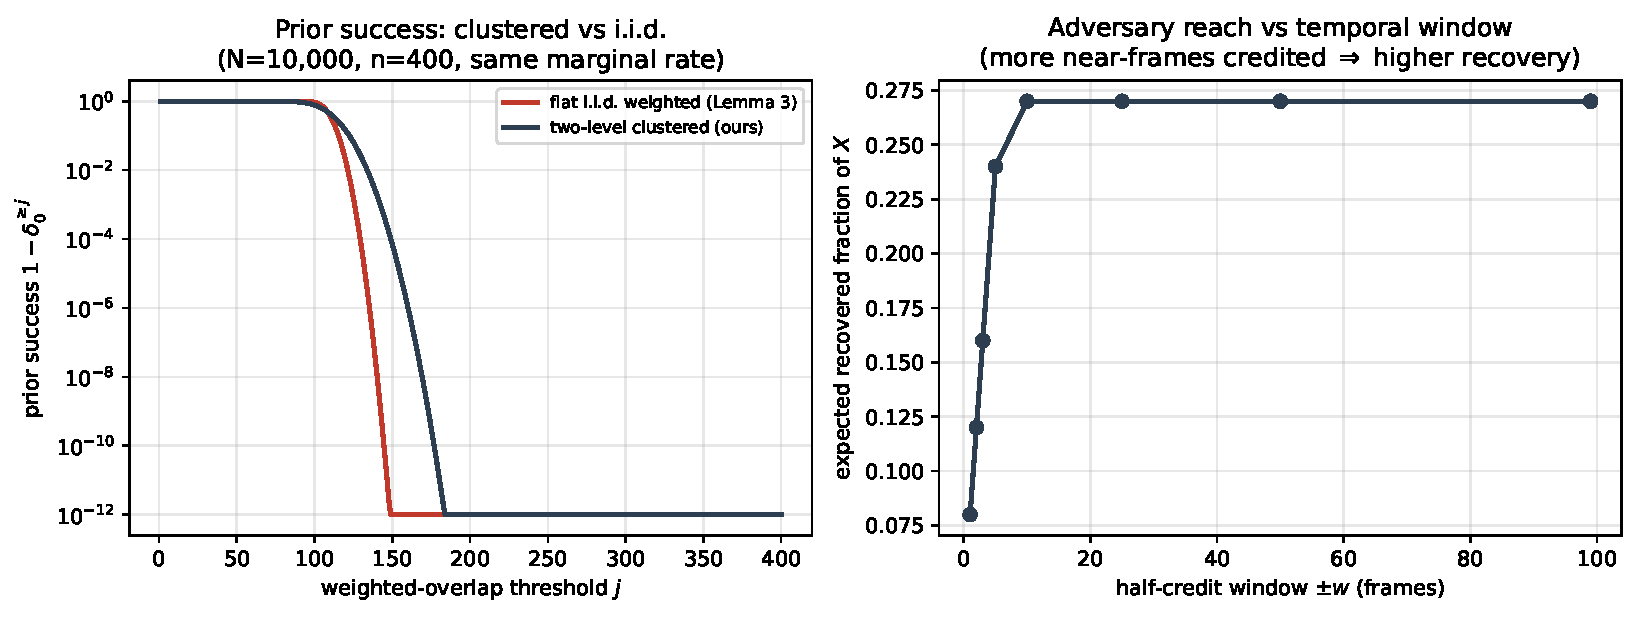
\includegraphics[width=\linewidth]{fig_two_level_prior.pdf}
\caption{Two-level clustered prior vs.\ the flat i.i.d.\ prior (Lemma~3). Left: at matched marginal rate and half-credit mass, the clustered prior (dark) has a far heavier upper tail than the i.i.d.\ prior (red), so it is the tail---not the mean---that an i.i.d.\ calibration under-protects. Right: the adversary's expected recovered fraction of the truth set grows monotonically with the half-credit temporal window.}
\label{fig:two_level}
\end{figure}

\section{Weight-Dependent Noise Calibration}

In this section, we connect the weighted temporal membership inference framework to noise calibration rules for learnable obfuscation mechanisms of the form $\mathcal{M}(X) = \Pi M_{\mathrm{mix}} X W + B$, combining mixing, permutation, masking, and additive noise. Our goal is to determine how much additional noise is required when the adversary receives graded (fractional-weight) credit for near-miss predictions.

\subsection{Mutual Information Bounds under Mixing and Masking}

We recall the key mutual information bounds from~\cite{xiao2024formal} that serve as the starting point for our calibration analysis.

\begin{theorem}[Inference Regarding Entire Set $X$; {\cite[Theorem~2]{xiao2024formal}}]
\label{thm:mi_masking}
When $W \in \mathbb{R}^{d_0 \times d}$ and $B \in \mathbb{R}^{n \times d}$ are two independent random matrices, where each entry of $W$ is i.i.d.\ $\mathcal{N}(0,1)$ and each column of $B$ is i.i.d.\ $\mathcal{N}(0, \Sigma_B)$ for some non-singular $\Sigma_B$, then for $X$ consisting of $n$ randomly generated data points,
\begin{equation}
\label{eq:mi_masking_bound}
\MI(X; XW + B) \le \frac{d}{2} \min \{ \mathrm{(I)}, \mathrm{(II)} \},
\end{equation}
where $\Sigma_X = XX^T$, $\Sigma_{X,B} = XX^T + \Sigma_B$, $X'$ is an independent copy of $X$, and
\begin{align*}
\mathrm{(I)} &:= \mathbb{E}_{X,X'}\!\left[
\mathrm{Tr}\!\left(
\Sigma_{X,B}^{-1}\Sigma_{X',B}
\right) - n
\right], \\
\mathrm{(II)} &:= \log \det\!\left(
\mathbb{E}_X\!\left[
I_n + \Sigma_B^{-1}\Sigma_X
\right]
\right)
- \mathbb{E}_X\!\left[
\log \det\!\left(
I_n + \Sigma_B^{-1}\Sigma_X
\right)
\right].
\end{align*}
\end{theorem}

When isotropic noise $\Sigma_B = \sigma I_n$ is used, the bound specializes as follows.

\begin{corollary}[Isotropic noise]
\label{cor:thm2_isotropic}
Under the setting of Theorem~\ref{thm:mi_masking} with $\Sigma_B = \sigma I_n$,
\begin{equation*}
\MI(X; XW + B) \;\le\; \frac{d}{2} \min \{ \mathrm{(I)}, \mathrm{(II)} \},
\end{equation*}
where
\begin{align*}
\mathrm{(I)} &:= \mathbb{E}_{X,X'}\!\left[
\mathrm{Tr}\!\left(
(XX^\top + \sigma I_n)^{-1}(X'X'^\top + \sigma I_n)
\right) - n
\right], \\
\mathrm{(II)} &:= \log \det\!\left(
\mathbb{E}_X\!\left[
I_n + \tfrac{1}{\sigma}\Sigma_X
\right]
\right)
- \mathbb{E}_X\!\left[
\log \det\!\left(
I_n + \tfrac{1}{\sigma}\Sigma_X
\right)
\right].
\end{align*}
\end{corollary}

\paragraph{Mixing and permutation bounds.}
\cite{xiao2024formal} further show (their Theorems~4--5) that when data mixing $M_{\mathrm{mix}}$ and permutation $\Pi$ are applied prior to masking and noise, the mutual information bounds~\eqref{eq:mi_masking_bound} hold with $X$ replaced by $\tilde{X} = \Pi M_{\mathrm{mix}} X$. The Type~(I) and~(II) bounds become functions of $\tilde{X}\tilde{X}^T$ rather than $XX^T$. Mixing stabilizes the Gram matrix by averaging over $k$ elements per class in each mixed sample, making $\tilde{X}\tilde{X}^T$ less sensitive to individual datapoint substitutions; permutation eliminates ordering-dependent instabilities. Together, these reduce the mutual information bound by up to an order of magnitude relative to masking alone (see Figure~1 and Tables~1--5 of~\cite{xiao2024formal}).

Mutual information is a property of joint distribution $(X, \mathcal{M}(X))$ and does not depend on the adversary's reward structure. Therefore, all mutual information bounds from~\cite{xiao2024formal}, including those incorporating mixing and permutation, hold unchanged in the weighted inference setting. The weight resolution affects only the adversary's \emph{prior success probability}, which enters through a separate factor in the adversary's success bound. We formalize this separation in the theorems below.

\subsection{Noise Calibration under Half-Integer Weights}

We first recall the adversary success bound from Lemma~\ref{lem:membership-hardness}, which is an adaptation of~\cite[Corollary~1]{xiao2024formal}. For any processing mechanism $\mathcal{M}$, the average membership success there is bounded by a single un-factored sum,
\[
1 - \bar{\delta}
\;\le\;
\sum_{j=1}^{n}
\frac{\MI(X;\mathcal{M}(X)) + (\log 2)/n}{D_j},
\qquad
D_j := -\log\!\big(1-\delta_0^{\ge j}\big),
\]
where $\delta_0^{\ge j}$ is the optimal a priori probability that a random guess achieves weighted overlap at least $j$, obtained in closed form from the stratified-hypergeometric distribution of the overlap between two independent $n$-subsets of the $c$-category universe. Since the numerator is independent of $j$, it factors out of the sum, giving the equivalent form
\begin{equation}
\label{eq:success_bound_recall}
\begin{gathered}
1 - \bar{\delta}
\;\le\;
\big(\MI(X;\mathcal{M}(X)) + (\log 2)/n\big)\cdot C, \\
C := \sum_{j=1}^{n} \frac{1}{D_j}.
\end{gathered}
\end{equation}
This factoring isolates the dependence of the bound on the adversary's reward structure: the mutual-information term depends only on the mechanism, while $C$ depends only on the weight structure through $\delta_0^{\ge j}$. Changing the weight resolution from integer to $1/m$ modifies $D_j$, and therefore $C$, but leaves $\MI(X;\mathcal{M}(X))$ unchanged. This separation reduces the calibration arguments below to comparisons of the ratio $C_{\mathrm{int}}/C_{1/m}$.

Under integer weights, $\delta_0^{\ge j}$ is determined by the standard hypergeometric distribution (Corollary~1), yielding $C_{\mathrm{int}}$. Under half-integer weights, Lemma~3 gives strictly larger prior success probabilities, yielding $C_{\mathrm{half}} > C_{\mathrm{int}}$. The following theorem determines the noise required to neutralize this increase.

\begin{theorem}[Half-integer noise calibration]
\label{thm:half_int_calibration}
Consider the mechanism $\mathcal{M}(X) = XW + B$ with $W$ having i.i.d.\ $\mathcal{N}(0,1)$ entries and $B$ having i.i.d.\ $\mathcal{N}(0,\sigma)$ entries. Let $C_{\mathrm{int}}$ and $C_{\mathrm{half}}$ denote the prior constants in~\eqref{eq:success_bound_recall} under integer and half-integer weights, respectively. Suppose that under integer weights with noise variance $\sigma_{\mathrm{int}}$, the adversary's success is bounded by
\[
1 - \bar{\delta}_{\mathrm{int}}
\;\le\;
\big(\MI_{\mathrm{int}} + \log 2\big)\, C_{\mathrm{int}},
\]
where $\MI_{\mathrm{int}} := \frac{d}{2}\min\{(I_{\sigma_{\mathrm{int}}}),(II_{\sigma_{\mathrm{int}}})\}$ is the mutual information upper bound from Theorem~\ref{thm:mi_masking}.

Then the adversary's success under half-integer weights is no larger than $1 - \bar{\delta}_{\mathrm{int}}$ provided the noise variance $\sigma_{\mathrm{half}} \ge \sigma_{\mathrm{int}}$ satisfies
\begin{equation}
\label{eq:half_calibration}
\frac{d}{2}\min\{(I_{\sigma_{\mathrm{half}}}),(II_{\sigma_{\mathrm{half}}})\}
\;\le\;
\big(\MI_{\mathrm{int}} + \log 2\big)\,\frac{C_{\mathrm{int}}}{C_{\mathrm{half}}}
\;-\; \log 2.
\end{equation}
Moreover, when mixing and permutation are applied, the same condition holds with the Type~(I) and~(II) bounds evaluated on $\tilde{X} = \Pi M_{\mathrm{mix}} X$ in place of $X$.
\end{theorem}

\begin{proof}
Under half-integer weights, the adversary's success bound~\eqref{eq:success_bound_recall} becomes
\[
1 - \bar{\delta}_{\mathrm{half}}
\;\le\;
\big(\MI_{\mathrm{half}} + \log 2\big)\, C_{\mathrm{half}},
\]
where $\MI_{\mathrm{half}}$ is the mutual information upper bound at noise level $\sigma_{\mathrm{half}}$. We require $1 - \bar{\delta}_{\mathrm{half}} \le 1 - \bar{\delta}_{\mathrm{int}}$, i.e.,
\[
\big(\MI_{\mathrm{half}} + \log 2\big)\, C_{\mathrm{half}}
\;\le\;
\big(\MI_{\mathrm{int}} + \log 2\big)\, C_{\mathrm{int}}.
\]
Rearranging for $\MI_{\mathrm{half}}$:
\[
\MI_{\mathrm{half}}
\;\le\;
\big(\MI_{\mathrm{int}} + \log 2\big)\,\frac{C_{\mathrm{int}}}{C_{\mathrm{half}}}
\;-\; \log 2.
\]
Since $C_{\mathrm{half}} > C_{\mathrm{int}}$ (because $\delta_{0,\mathrm{half}}^{\ge j} \ge \delta_{0,\mathrm{int}}^{\ge j}$ for all $j$ by Lemma~3, which gives $D_{j,\mathrm{half}} \le D_{j,\mathrm{int}}$), the right-hand side is strictly less than $\MI_{\mathrm{int}}$. By Theorem~\ref{thm:mi_masking}, the mutual information bound $\frac{d}{2}\min\{(I_\sigma),(II_\sigma)\}$ is monotonically decreasing in $\sigma$. Therefore, there exists $\sigma_{\mathrm{half}} \ge \sigma_{\mathrm{int}}$ satisfying~\eqref{eq:half_calibration}, and any such $\sigma_{\mathrm{half}}$ ensures $1 - \bar{\delta}_{\mathrm{half}} \le 1 - \bar{\delta}_{\mathrm{int}}$.

For the mixing extension, mutual information is a divergence between the joint distribution $(X, \mathcal{M}(X))$ and the product of marginals, and hence depends only on the mechanism and data distribution, not on the adversary's reward structure. The Type~(I) and~(II) bounds from Theorems~4--5 of~\cite{xiao2024formal} therefore apply without modification under half-integer weights, with $X$ replaced by $\tilde{X}$.
\end{proof}

\subsection{Noise Calibration under \texorpdfstring{$1/m$}{1/m}-Resolution Weights}

We now extend the calibration to arbitrary fractional-weight resolution.

\begin{theorem}[General $1/m$-resolution noise calibration]
\label{thm:general_m_calibration}
In the same setting as Theorem~\ref{thm:half_int_calibration}, let $m \ge 2$ be an integer specifying the weight resolution, so that weights take values in $\{0, 1/m, 2/m, \dots, 1\}$. Let $C_{1/m}$ denote the prior constant in~\eqref{eq:success_bound_recall} computed using the $1/m$-resolution prior success probabilities from Lemma~4. Then:
\begin{enumerate}[label=(\roman*)]
    \item $C_{1/m} \ge C_{\mathrm{int}}$, with equality if and only if $M_r = 0$ for all $1 \le r \le m-1$ (no fractional-weight elements).

    \item The adversary's success under $1/m$-resolution weights is no larger than $1 - \bar{\delta}_{\mathrm{int}}$ provided the noise variance $\sigma_{1/m} \ge \sigma_{\mathrm{int}}$ satisfies
    \begin{equation}
    \label{eq:m_calibration}
    \frac{d}{2}\min\{(I_{\sigma_{1/m}}),(II_{\sigma_{1/m}})\}
    \;\le\;
    \big(\MI_{\mathrm{int}} + (\log 2)/n\big)\,\frac{C_{\mathrm{int}}}{C_{1/m}}
    \;-\; (\log 2)/n.
    \end{equation}

    \item Whenever $M_r > 0$ for some $1 \le r \le m-1$, the inequality in part~(i) is strict, and the required noise variance satisfies $\sigma_{1/m} > \sigma_{\mathrm{int}}$: the presence of any fractional-weight elements forces strictly more noise than the integer-weight baseline.
\end{enumerate}
\end{theorem}

\begin{proof}
\textbf{Part (i).} Fix a threshold $j \in \{1,\dots,n\}$. For any realization of the count vector $(k_0,\dots,k_m)$ drawn from the $1/m$-resolution multivariate hypergeometric of Lemma~4, the integer overlap on the same $\widehat{X}$ equals $W_{\mathrm{int}} = k_m$, whereas the $1/m$-resolution overlap is
\[
W_{1/m}
\;=\;
k_m + \sum_{r=1}^{m-1}\frac{r}{m}k_r
\;\ge\; k_m
\;=\; W_{\mathrm{int}},
\]
with strict inequality whenever some $k_r > 0$ for $1 \le r \le m-1$. Hence $\{W_{\mathrm{int}} \ge j\} \subseteq \{W_{1/m} \ge j\}$ as events on the same probability space, so
\[
1 - \delta_{0,1/m}^{\ge j}
\;\ge\;
1 - \delta_{0,\mathrm{int}}^{\ge j},
\]
which gives $D_{j,1/m} \le D_{j,\mathrm{int}}$ for every $j$, and summing yields $C_{1/m} \ge C_{\mathrm{int}}$. Equality holds throughout iff $k_r = 0$ almost surely for all $1 \le r \le m-1$, i.e.\ iff $M_r = 0$ for those $r$.

\textbf{Part (ii).} By~\eqref{eq:success_bound_recall} the adversary's success under $1/m$-resolution weights satisfies
\[
1 - \bar{\delta}_{1/m}
\;\le\;
\big(\MI_{1/m} + (\log 2)/n\big)\, C_{1/m}.
\]
Requiring $1 - \bar{\delta}_{1/m} \le 1 - \bar{\delta}_{\mathrm{int}} \le (\MI_{\mathrm{int}} + (\log 2)/n)\, C_{\mathrm{int}}$ and rearranging yields
\[
\MI_{1/m}
\;\le\;
\big(\MI_{\mathrm{int}} + (\log 2)/n\big)\,\frac{C_{\mathrm{int}}}{C_{1/m}}
\;-\; (\log 2)/n.
\]
Since $C_{1/m} \ge C_{\mathrm{int}}$ by part~(i), the right-hand side is at most $\MI_{\mathrm{int}}$. By Theorem~\ref{thm:mi_masking} the mutual information bound is monotonically decreasing in $\sigma$, so there exists $\sigma_{1/m} \ge \sigma_{\mathrm{int}}$ satisfying~\eqref{eq:m_calibration}.

\textbf{Part (iii).} Under the hypothesis $M_r > 0$ for some $1 \le r \le m-1$, the event-inclusion in part~(i) is strict with positive probability, so $C_{1/m} > C_{\mathrm{int}}$. The right-hand side of~\eqref{eq:m_calibration} is therefore strictly less than $\MI_{\mathrm{int}}$, and strict monotonicity of the mutual information bound in $\sigma$ (Theorem~\ref{thm:mi_masking}) forces $\sigma_{1/m} > \sigma_{\mathrm{int}}$.
\end{proof}

Theorems~\ref{thm:half_int_calibration} and~\ref{thm:general_m_calibration} make precise the privacy cost of weighted inference. The ratio $C_{\mathrm{int}}/C_{1/m} < 1$ quantifies how much the adversary's prior advantage increases at resolution $1/m$; the mechanism must compensate by reducing mutual information by the same factor. When data mixing is applied, the mutual information is already reduced (per the bounds of~\cite{xiao2024formal}), partially offsetting the increased prior. The privacy--utility relationship thus depends on the interplay between mixing intensity (which reduces $\MI$) and weight resolution (which increases $C$). A direct consequence is that even modest relaxation of the correctness criterion---from exact membership ($m=1$) to half-integer proximity ($m=2$)---can require substantially more noise to maintain equivalent privacy, motivating the experimental comparison in Section~\ref{sec:experiments}.

\subsection{Noise Design under Dependence}
\label{subsec:correlated_noise}

Independent per-frame noise is natural when frames are classified individually, but a model that jointly processes a clip---and, dually, an adversary that pools evidence across a clip's frames---is not best countered by independent noise. Consider a mechanism whose noise is $B_r = \sqrt{1-f}\,\varepsilon_r + \sqrt{f}\,\eta_{c(r)}$, where $\varepsilon_r$ is an independent per-frame draw and $\eta_c$ is a per-clip shared draw; the total per-frame variance is $\sigma^2$ for any mixing fraction $f \in [0,1]$, so the noise budget is unchanged. Under a correlation-aware attack (Algorithm~\ref{alg:aware}), the shared component $\eta_c$ sums \emph{coherently} across a clip's frames and cannot be averaged out, whereas independent noise partially cancels. We show on synthetic AR(1) clips (Section~\ref{subsec:correlation_aware_exp}) that at matched budget, moving from $f=0$ (i.i.d.) to $f=1$ (fully clip-shared) reduces the pooling adversary's success while leaving the blind adversary unaffected. In that controlled setting, correlated noise is the better design for the joint-processing threat at no extra budget; we have not yet validated this defense on real UCF-101, where the random per-clip frame sampling of our evaluation mutes the intra-clip correlation the pooling attack exploits.

\section{Experiments}
\label{sec:experiments}

We empirically evaluate the theoretical results of Sections~4 and~5, primarily on the UCF-101 action recognition dataset~\cite{soomro2012ucf101} and, for the correlation-aware analysis, complemented by a controlled synthetic study. Section~\ref{subsec:exp_setup} describes the pipeline shared by the downstream classifier and the temporal membership inference attack. Section~\ref{subsec:numerical_validation} numerically evaluates Theorems~\ref{thm:half_int_calibration} and~\ref{thm:general_m_calibration} on the universe used in Lemma~3's visualization. Section~\ref{subsec:mia_operating_point} reports empirical attack scores at a representative operating point against closed-form chance baselines, Section~\ref{subsec:correlation_aware_exp} evaluates the correlation-aware attack and correlated noise---combining a controlled synthetic study that isolates the correlation with a real UCF-101 evaluation---and Section~\ref{subsec:utility} reports downstream classifier accuracy across the noise sweep.

\subsection{Experimental Setup}
\label{subsec:exp_setup}

Our experimental design follows the protocol of~\cite{xiao2024formal}: the data owner applies the obfuscation mechanism to features that have already been embedded by an ImageNet-pretrained backbone, so that the embedding plays the role of an implicit random projection $W$ in Algorithm~1 of~\cite{xiao2024formal}. This pipeline mitigates the ill-conditioning of raw data matrices that would otherwise make the mutual information bounds of Theorem~\ref{thm:mi_masking} (and Theorems~4--5 of~\cite{xiao2024formal}) numerically vacuous; similar to prior work, we adopt a ResNet-18 backbone on UCF-101 frames. The temporal membership inference attack additionally evaluates the explicit form of the mechanism on flattened pixels, so the projection $W$ is also instantiated and analyzed directly.

We evaluate on UCF-101 split~1, an action recognition benchmark with $c = 101$ classes containing $9{,}537$ training clips and $3{,}783$ test clips. To make the per-clip frame-index universe uniform across the dataset, every clip is preprocessed by a fixed-length trim: clips with fewer than $L = 100$ frames are dropped, and longer clips are truncated to their first $L$ frames. After trimming, $7{,}954$ training clips are retained.  Each clip is embedded by drawing $T = 16$ frame indices uniformly without replacement from $[0, L)$, resizing each frame to $224 \times 224$, and passing it through a pretrained ResNet-18 backbone (ImageNet-1K weights, classification head removed) to produce a per-clip representation of shape $(T, d_0)$ with $d_0 = 512$, L2-normalized along the feature dimension. The choice of random rather than deterministic sampling reflects a deliberate trade-off between utility and privacy. Deterministic sampling (e.g., \texttt{linspace} over $[0, L)$) is the natural choice for the downstream classifier, since fixed indices give the temporal model consistent frame coverage across clips and let it exploit the temporal structure of action sequences. However, fixed indices also collapse the index-inference task: an adversary who knows the sampling rule recovers the true frame indices for every clip without observing $\mathcal{M}(X)$ at all. Random per-clip sampling restores a meaningful inference task. We use the same random sampling rule for the downstream classifier and the temporal membership inference attack so that the two pipelines see the same data distribution. Overall, the trimming and sampling define the temporal membership inference universe of size $|U| = 7{,}954 \times 16 = 127{,}264$ candidate (clip, index) pairs.

Both the obfuscated classifier and its no-obfuscation baseline train on a stratified subset of exactly $50$ clips per class ($n = 5{,}050$ total), share the same temporal classifier---a Transformer encoder ($2$ layers, $8$ heads, $d_{\mathrm{ff}} = 512$, dropout $0.1$, learnable \texttt{[CLS]} token, learned positional embeddings, applied to the $(T, d_0)$ frame-embedding sequence and read off from the \texttt{[CLS]} token)---and use the same Adam optimizer (learning rate $10^{-3}$, batch size $64$, $50$ epochs). The obfuscation mechanism is the one defined in Section~\ref{sec:preliminary}; the downstream classifier sees $\mathcal{M}(X) = \Pi_1 M_{\mathrm{mix}} X + B$ on cached per-frame embeddings (the ResNet-18 frame encoder absorbs the projection $W$, so no further $W$ is applied), and the temporal membership inference attack uses the explicit form $T_X(X) = \Pi_1 M_{\mathrm{mix}} X W + B$ with $W \in \mathbb{R}^{d_0 \times d}$, $W_{ij} \sim \mathcal{N}(0, 1/d)$, $d = 500$, applied to flattened grayscale frames of size $112 \times 112$. Class-$k$ mixing $M_{\mathrm{mix}}$ produces $m = c^2 = 10{,}201$ mixed samples by sampling, for each ordered class pair $(i, j) \in [c] \times [c]$, $k$ clip-embeddings from class $i$ and $k$ from class $j$ and averaging them frame-by-frame; the soft target is one-hot on class $i$ when $i = j$, and places mass $1/2$ on each class otherwise. For $k = 0$ no mixing is applied and the classifier is trained on the $n = 5{,}050$ raw embeddings with one-hot targets. Soft targets are passed directly to a soft-label cross-entropy loss without collapsing to hard labels.

Figure~\ref{fig:visual_obfuscation} visualizes the mechanism in pixel space at illustrative parameters $(k, \sigma) = (5, 0.1)$, with the projection $W$ omitted for visual clarity.

\begin{figure}[!htbp]
\centering
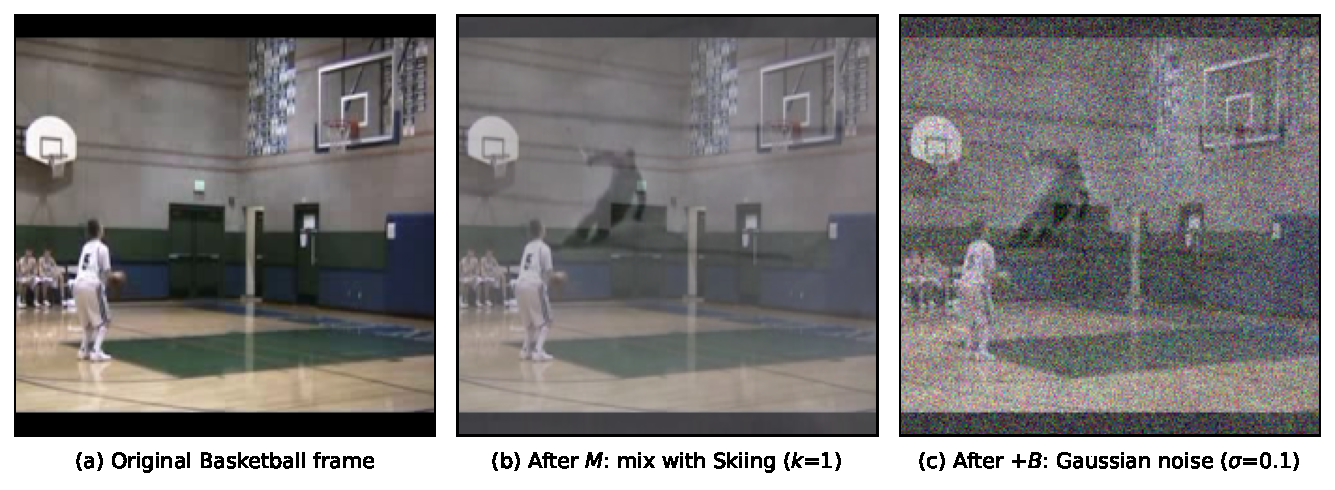
\includegraphics[width=\linewidth]{figure5_visual_obfuscation_pixel.pdf}
\caption{Pixel-space visualization of the obfuscation pipeline at $(k, \sigma) = (5, 0.1)$.}
\label{fig:visual_obfuscation}
\end{figure}

\paragraph{The obfuscation mechanism, explicitly.}
Algorithm~\ref{alg:mech} states the release the classifier and adversary observe, making explicit the line at which the noise level $\sigma$ enters.

\begin{algorithm}[t]
\caption{Obfuscation mechanism $\mathcal{M}$ (per~\cite{xiao2024formal}, made explicit)}
\label{alg:mech}
\begin{algorithmic}[1]
\Require dataset $X\in\mathbb{R}^{n\times d}$, labels $Y$, mixing $k$, projection dim $d'$, noise level $\sigma$
\Ensure  released $(\mathcal{M}(X), \tilde Y)$
\State $M_{\mathrm{mix}} \gets$ class-$k$ mixing matrix from $Y$ \Comment{averages $k$ same- and $k$ cross-class rows}
\State $W \sim \mathcal{N}(0, 1/d')^{d\times d'}$ \Comment{fixed random projection}
\State $\Pi_1 \gets$ random row permutation;\; $\Pi_2 \gets$ random label permutation
\State $B \sim \mathcal{N}(0,\sigma^2)^{m\times d'}$ \Comment{$\sigma$ enters HERE: additive Gaussian noise}
\State \textbf{return} $\mathcal{M}(X) = \Pi_1 M_{\mathrm{mix}} X W + B$,\;\; $\tilde Y = \Pi_1 M_{\mathrm{mix}} Y \Pi_2$
\end{algorithmic}
\end{algorithm}

\subsection{Numerical Evaluation of Theorems~\ref{thm:half_int_calibration} and~\ref{thm:general_m_calibration}}
\label{subsec:numerical_validation}

\begin{table}[!htbp]
\centering\small
\caption{Results for Analyses in Theorems~\ref{thm:half_int_calibration} and~\ref{thm:general_m_calibration}. The prior constant $C_{\mathrm{half}}$ under half-integer weights exceeds the integer baseline $C_{\mathrm{int}}$ by $31\times$, forcing a $5.6\times$ noise increase.}
\label{tab:calibration}
\begin{tabular}{lrrr}
\toprule
Weight rule & $C$ & $C/C_{\mathrm{int}}$ & $\sigma/\sigma_{\mathrm{int}}$ \\
\midrule
Integer ($C_{\mathrm{int}}$)      & $20.77$  & $1.0000$  & $1.0000$ \\
Half-integer ($C_{\mathrm{half}}$) & $651.8$  & $31.384$  & $5.602$ \\
\bottomrule
\end{tabular}
\end{table}

Table~\ref{tab:calibration} numerically evaluates Theorems~\ref{thm:half_int_calibration} and~\ref{thm:general_m_calibration} on the universe used in Lemma~3's visualization (Figure~\ref{fig:prior_success}, $N = 1000$, $n = 50$, $m = 100$, $q = 0.05$). The constant $C := \sum_{j=1}^n 1/D_j$ with $D_j = -\log(1 - \delta_0^{\ge j})$ is the prior-dependent factor in the adversary success bound of Lemma~\ref{lem:membership-hardness}, and the ratio $C_{\mathrm{half}}/C_{\mathrm{int}}$ controls how much additional noise the mechanism must inject to preserve the same MI-based privacy guarantee under half-integer scoring (Theorem~\ref{thm:half_int_calibration}).

The numerical evaluation makes two contributions concrete. First, it confirms that the strict inequality $C_{\mathrm{half}} > C_{\mathrm{int}}$ predicted by Theorem~\ref{thm:general_m_calibration} part~(i) is not a vacuous one: at half-integer resolution on this universe, $C$ inflates by $31\times$, so even the simplest fractional-weight relaxation incurs an order-of-magnitude penalty on the prior factor. Second, translating the inflation through the $\mathrm{MI} \sim 1/\sigma^2$ approximation of Theorem~\ref{thm:mi_masking} gives a multiplicative noise inflation of $\sqrt{C_{\mathrm{half}}/C_{\mathrm{int}}} \approx 5.6\times$ to maintain the same MI-based bound: the privacy cost of weighted inference is a large constant factor in $\sigma$, not a marginal correction.

\subsection{Empirical Temporal Membership Inference}
\label{subsec:mia_operating_point}

We instantiate the temporal membership inference attack at the operating point $(k, \sigma) = (1, 0.1)$ and report two attack scenarios against the closed-form random-guess and no-obfuscation baselines. We focus on a single operating point rather than a $\sigma$-sweep on the privacy axis because the informed-adversary attacks succeed in absolute terms across the entire noise range we evaluate (see Appendix~\ref{app:sigma_sweep} for the full sweep results); the $\sigma$ sweep is therefore reported on the utility axis in Section~\ref{subsec:utility}. The attacks share one likelihood-ratio scoring core, adapted from the Likelihood Ratio Attack (LiRA) of Carlini \textit{et al.}~\cite{carlini2022firstprinciples}. LiRA scores each candidate by the log-likelihood ratio of two Gaussian hypotheses---``the candidate was a member'' versus ``the candidate was a non-member''---under the noise model of the release. We instantiate this idea in our obfuscation setting as follows: the attacker forms a residual $r := o - \mathcal{M}(X_{\mathrm{cf}})$ between the observed release $o$ and the mechanism applied to a same-class counterfactual dataset $X_{\mathrm{cf}}$, and ranks each candidate $c$ by
\[
\mathrm{LR}(c) = \frac{r \cdot \Delta_c}{\sigma^2} - \frac{1}{2} \frac{\|\Delta_c\|^2}{\sigma^2},
\]
where $\Delta_c$ is the per-candidate predicted difference between the two hypotheses, evaluated at $c$'s mixed-row positions. This is the log-likelihood ratio of the two Gaussian hypotheses under additive noise of variance $\sigma^2$, modulo a constant that does not affect ranking.

 The two attacks differ only in which set of candidates is ranked and how the top-ranked guesses are scored. \emph{Attack~1 (index inference)} models an \textit{informed} adversary who knows the target clip and is asked to recover its frame indices: it ranks the $L = 100$ candidate frame indices for the target clip and emits the top-$T$, scored under a half-credit rule with a $\pm 2$-frame temporal-proximity window: an exact (clip, index) match earns $1$, a same-clip guess within $\pm 2$ of any true frame earns $0.5$, otherwise $0$.
\emph{Attack~2 (frame-level temporal membership inference)} models an \textit{uninformed} adversary with no side information about clip or class: it rank-orders a uniformly random subsample $U_2$ of $|U_2| = 2{,}016$ candidate (clip, index) pairs drawn from the full universe $|U| = 127{,}264$, with the $T = 16$ true target rows always included in $U_2$, and emits the top-$T$ guesses under the same half-credit window rule as Attack~1. The subsample is a tractability concession---scoring all $127{,}264$ candidates per Monte Carlo trial dominates per-cell cost---and does not give the adversary side information about which (clip, index) pairs are members: the truth is buried in $U_2$ alongside random distractors, and the chance baseline below is computed against the actual pool the adversary scored. Algorithm~\ref{alg:blind} states the blind (per-frame) form of this attack.

\begin{algorithm}[t]
\caption{Blind temporal MIA (Attack~2, the i.i.d.\ adversary)}
\label{alg:blind}
\begin{algorithmic}[1]
\Require release $\mathcal{M}(X)$, candidate pool $P$ of (clip, index) rows, target size $T$
\Ensure  $T$ guessed (clip, index) pairs
\State for each candidate $r\in P$: $\ell_r \gets \textsc{LiRA}(r; \mathcal{M}(X))$ \Comment{per-frame likelihood ratio, scored independently}
\State \textbf{return} the $T$ candidates with the largest $\ell_r$
\end{algorithmic}
\end{algorithm}

\begin{table}[t]
\centering\small
\caption{Empirical temporal membership inference scores at $(k, \sigma) = (1, 0.1)$. The Empirical column reports the mean over $n = 50$ samples, with the standard error $\mathrm{std}/\sqrt{n}$ in parentheses. Full sweep of parameters is available in Appendix~\ref{app:sigma_sweep}.}
\label{tab:operating_point}
\resizebox{1\columnwidth}{!}{%
\begin{tabular}{lrrr}
\toprule
Attack & Empirical & No Obfuscation & Random Baseline \\
\midrule
Attack~1 (informed)        & $0.404\,(0.02)$ & $0.460\,(0.019)$ & $0.373$ \\
Attack~2 (uninformed)  & $0.439\,(0.05)$ & $0.835\,(0.039)$&  $0.0079$ \\
\bottomrule
\end{tabular}
}
\end{table}

\paragraph{Random-guess baselines.}
The Random Baseline column in Table~\ref{tab:operating_point} is computed in closed form, separately for each attack, against the candidate pool the attack actually scored. \emph{Attack~1} averages over guesses uniformly distributed in the $L = 100$-frame target clip; under the $\pm 2$-window half-credit rule, the per-guess expected score is
\[
\frac{T}{L} + \frac{1}{2}\left(\frac{\mathbb{E}\lvert N\rvert}{L} - \frac{T}{L}\right) \;\approx\; 0.373,
\]
\emph{Attack~2} averages over guesses uniformly drawn from the subsample $U_2$. Because the universe contains only $T$ sampled (clip, index) rows per clip, every row in $U_2$ that lies in the target clip is one of the $T$ true target rows; there are no ``near, not exact'' rows in $U_2$ to receive half credit. Under the $\pm 2$-window rule, the per-guess expected score therefore reduces to the exact-match probability,
\[
\frac{T}{|U_2|} \;=\; \frac{16}{2{,}016} \;\approx\; 0.0079.
\]

Table~\ref{tab:operating_point} reports the two attack scores against these baselines, evaluated over $n_{\mathrm{targets}} = 10$ target clips with $n_{\mathrm{trials}} = 5$ Monte Carlo trials each ($n = 50$ samples per metric).

The two attacks together demonstrate that the obfuscation mechanism reduces privacy leakage relative to a no-obfuscation baseline but does not eliminate it: the obfuscated attack scores (Empirical column) fall below the no-obfuscation scores, yet remain non-trivially above chance, so residual leakage about the underlying clips and frames persists in this regime, even when the adversary has no side information (Attack~2). Results also show that obfuscation is substantially more effective for an uninformed adversary (i.e., the more realistic scenario). This is consistent with, but does not numerically certify, the upper bound of Lemma~\ref{lem:membership-hardness}: that lemma guarantees the existence of a finite gap between adversary success and~$1$ as a function of $\MI(X; \mathcal{M}(X))$, which Theorem~\ref{thm:mi_masking} controls through the mechanism's mixing and additive noise. We do not claim to empirically verify the bound here---that would require a direct estimate of $\MI(X; \mathcal{M}(X))$, which we leave to future work (Section~\ref{sec:conclusion}). What this section establishes is operational: at a representative $(k, \sigma)$, the mechanism admits real residual leakage but does not saturate, and the leakage that the attacks detect is consistent with the bound's qualitative prediction. We also refer the reader to additional results and analysis in the Appendix.

\subsection{Correlation-Aware Attack and Correlated Noise}
\label{subsec:correlation_aware_exp}

Attacks~1 and~2 score each candidate frame independently, treating the universe as i.i.d.---the assumption our theory (Section~\ref{subsec:two_level}) argues is optimistic. We therefore evaluate a \emph{correlation-aware} adversary (Algorithm~\ref{alg:aware}) that pools the same per-frame likelihood-ratio evidence across a clip before deciding, mirroring the compound prior of Lemma~\ref{lem:two_level}: winning one clip delivers a block of correlated credit. Both adversaries observe the same release and use the same LiRA scores; they differ only in whether they exploit the clip structure.

\begin{algorithm}[t]
\caption{Correlation-aware temporal MIA}
\label{alg:aware}
\begin{algorithmic}[1]
\Require release $\mathcal{M}(X)$, candidate pool $P$ grouped by clip, target $T$
\Ensure  $T$ guessed (clip, index) pairs
\State for each $r\in P$: $\ell_r \gets \textsc{LiRA}(r; \mathcal{M}(X))$ \Comment{same per-frame scores as Alg.~\ref{alg:blind}}
\State for each clip $c$: $s_c \gets \sum_{r\in c}\ell_r$ \Comment{pool correlated evidence across the clip}
\State $c^\star \gets \arg\max_c s_c$ \Comment{identify the source clip}
\State \textbf{return} the $T$ highest-$\ell_r$ rows within $c^\star$ (fill from next clips if fewer than $T$)
\end{algorithmic}
\end{algorithm}

\paragraph{Controlled study.}
Because correlation in real video is uncontrolled, we first isolate its effect on synthetic clips whose intra-clip temporal correlation is a single dial $\rho \in [0,1)$: each clip is an AR(1) sequence with $\mathrm{Corr}(\text{frame}_s,\text{frame}_t) = \rho^{|s-t|}$, so $\rho=0$ is the i.i.d.\ model the theory assumes and $\rho \to 1$ is a nearly static video. Passing these through the same mechanism and LiRA scoring (Figure~\ref{fig:synthetic}), we find three effects. First, \emph{graded leakage is real}: the likelihood-ratio score of a \emph{non-member} frame rises as its temporal distance to the nearest member shrinks, with reach growing in $\rho$; at $\rho=0$ only members score above baseline, so the partial-credit reward the paper defines corresponds to measurable leakage. Second, at a fixed noise level the correlation-aware attack's source-clip identification rises from $0.75$ at $\rho=0$ to $1.00$ at $\rho \ge 0.9$, while the blind i.i.d.\ adversary lags ($0.05 \to 0.87$): correlation the flat model treats as absent is exactly what the attack exploits. Third, at matched noise budget, making the mechanism noise clip-correlated (Section~\ref{subsec:correlated_noise}) reduces the pooling adversary's success from $0.29$ to $0.17$ while leaving the blind adversary unaffected, confirming that independent per-frame noise is not the right design for the joint-processing threat.

\begin{figure}[!htbp]
\centering
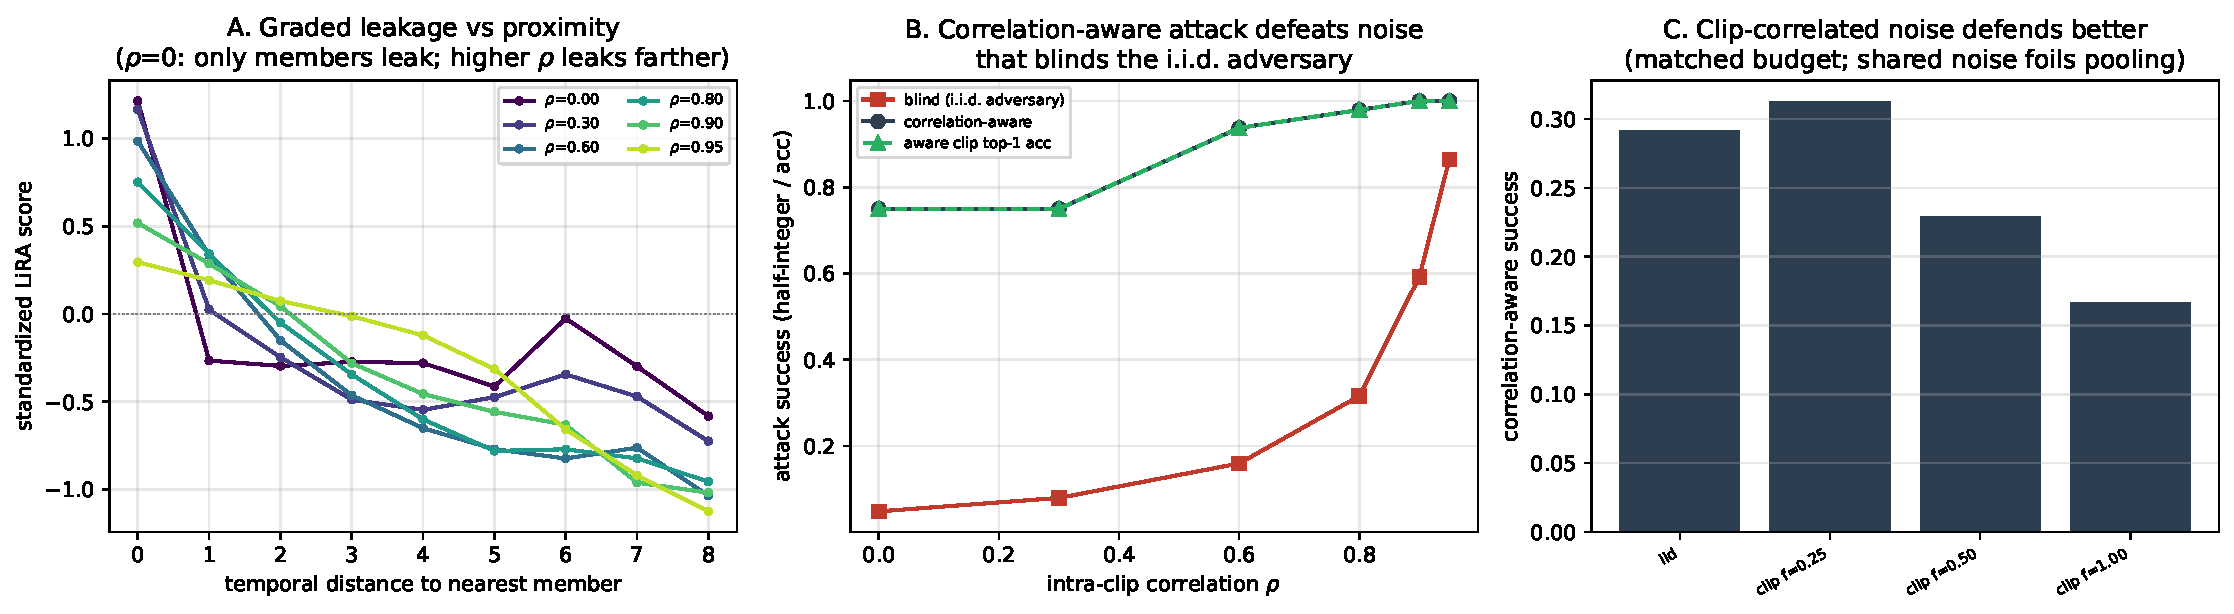
\includegraphics[width=\linewidth]{fig_synthetic_correlation.pdf}
\caption{Controlled-correlation study on synthetic AR(1) clips. Left: likelihood-ratio score vs.\ temporal distance to the nearest member; leakage is flat at $\rho=0$ and reaches farther as $\rho$ grows. Middle: the correlation-aware attack (and its clip-identification accuracy) defeats a noise level that blinds the i.i.d.\ adversary, with the advantage growing in $\rho$. Right: at matched budget, clip-correlated noise defends the pooling adversary better than i.i.d.\ noise.}
\label{fig:synthetic}
\end{figure}

\paragraph{On UCF-101.}
On real UCF-101, the correlation-aware attack identifies the source clip well above chance---top-$1$ accuracy $\approx 0.47$--$0.57$ out of $400$ candidate clips, against a $1/400$ random baseline. Source-clip identification is an intermediate diagnostic, however; the privacy-relevant comparison is against the blind attack, over which the correlation-aware attack gives only a small improvement in weighted recovery (positive at three of the four noise levels we evaluate). The effect is more modest than in the controlled study, and for an instructive reason: the random per-clip frame sampling of Section~\ref{subsec:exp_setup} scatters the $T=16$ members across the $L=100$-frame clip, weakening precisely the intra-clip correlation the attack exploits. The design choice that makes index inference a well-posed task (random sampling) therefore also mutes the correlation signal on real data; the synthetic study isolates the full effect. We report this tension explicitly rather than leaving it implicit.

\subsection{Utility}
\label{subsec:utility}

\begin{table}[t]
\centering\small
\caption{UCF-101 split-1 test accuracy across the $(k, \sigma)$ sweep.}
\label{tab:utility}
\begin{tabular}{ccrr}
\toprule
$k$ & $\sigma$ & Test Acc.\ (\%) & $\Delta$ vs.\ baseline (pp) \\
\midrule
\multicolumn{2}{c}{No obfuscation} & $60.19$ & --- \\
\midrule
$0$ & $0.01$ & $64.81$ & $+4.62$  \\
$0$ & $0.05$ & $72.35$ & $+12.16$ \\
$0$ & $0.10$ & $68.24$ & $+8.05$  \\
$0$ & $0.50$ & $30.54$ & $-29.64$ \\
\midrule
$1$ & $0.01$ & $70.00$ & $+9.82$  \\
$1$ & $0.05$ & $68.37$ & $+8.18$  \\
$1$ & $0.10$ & $66.60$ & $+6.42$  \\
$1$ & $0.50$ & $42.83$ & $-17.36$ \\
\midrule
$5$ & $0.01$ & $66.92$ & $+6.74$  \\
$5$ & $0.05$ & $66.67$ & $+6.48$  \\
$5$ & $0.10$ & $64.93$ & $+4.75$  \\
$5$ & $0.50$ & $43.95$ & $-16.23$ \\
\bottomrule
\end{tabular}
\end{table}

Table~\ref{tab:utility} reports test accuracy on UCF-101 split-1 across all twelve $(k, \sigma)$ configurations of the obfuscation mechanism, evaluated against a no-obfuscation baseline trained under the same random-sampling protocol; hard-argmax accuracy is computed on the raw test set with only the label permutation $\Pi_2$ inverted at evaluation. For $\sigma \le 0.10$, every obfuscated configuration exceeds the no-obfuscation baseline of $60.19\%$, with the peak ($+12.16$pp at $k = 0, \sigma = 0.05$) appearing in the low-noise interior; within this band the dependence on mixing intensity $k$ is weak and not strictly monotone. At $\sigma = 0.50$, utility collapses across all values of $k$, defining $\sigma \le 0.10$ as the mechanism's operable noise envelope.

The fact that several low-noise configurations \emph{exceed} the no-obfuscation baseline is consistent with class-$k$ mixing acting as a mild regularizer at small $\sigma$; we report this as an empirical observation rather than as a privacy contribution.

\paragraph{Connection to the calibration analysis.}
The utility sweep complements the prior-cost analysis of Section~\ref{subsec:numerical_validation} by quantifying the noise budget within which the calibration-required inflation $\sigma_{\mathrm{half}} \ge \sqrt{C_{\mathrm{half}}/C_{\mathrm{int}}} \cdot \sigma_{\mathrm{int}}$ of Theorems~\ref{thm:half_int_calibration} and~\ref{thm:general_m_calibration} could in principle be absorbed without sacrificing downstream accuracy. On the universe of Lemma~3's visualization, the required inflation is $5.6\times$, which would push an integer-weight operating point of $\sigma_{\mathrm{int}} = 0.05$ to $\sigma_{\mathrm{half}} \approx 0.28$---outside the operable band identified here. Whether this is a binding constraint in a specific deployment depends on the deployment-specific universe: the inflation factor is determined by the actual weight-class layout $(M_0, M_1, \dots, M_m)$, which controls $C_{\mathrm{half}}/C_{\mathrm{int}}$, and may be substantially smaller than the value computed on Lemma~3's universe.

Two further qualifications attach to the empirical comparison. First, the temporal membership inference evaluation in Section~\ref{subsec:mia_operating_point} ranks Attack~2 over a subsampled candidate pool of $|U_2| = 2{,}016$ rather than the full $|U| = 127{,}264$. This is an adversary-friendly choice taken for computational tractability; even under it, no attack we evaluated saturated at $\sigma = 0.05$, leaving real margin within the $\sigma \le 0.10$ envelope. Second, the calibration is stated for the MI-based bound, not for empirical attack success, so its quantitative force depends on how tight Theorem~\ref{thm:mi_masking}'s upper bound is in a given regime---a question we leave to the future-work directions of Section~\ref{sec:conclusion}. Together, the prior factor of Section~\ref{subsec:numerical_validation} and the utility envelope of this section identify the design quantities a practitioner needs to assess whether privacy and utility are simultaneously satisfiable for a target deployment.


\section{Conclusion}
\label{sec:conclusion}

This work extends the formal learnable obfuscation framework of~\cite{xiao2024formal} to temporally correlated video data through \emph{weighted temporal membership inference}, in which adversarial success is graded by semantic and temporal proximity rather than exact frame recovery. We derived closed-form multivariate hypergeometric expressions for the adversary's prior success probability under half-integer and general $1/m$-resolution weights (Lemmas~3 and~4) and showed that these priors strictly dominate their integer-weight counterpart. Beyond the reward, we modeled the dependence itself: a two-level clip-then-frame sampling process whose compound prior (Lemma~\ref{lem:two_level}) strictly generalizes the i.i.d.\ analysis and shows that clustered membership inflates the adversary's upper-tail success and the required noise. We then obtained noise calibration conditions (Theorems~\ref{thm:half_int_calibration} and~\ref{thm:general_m_calibration}) quantifying the additional noise required to preserve a target privacy guarantee under weighted proximity, with the mixing and permutation amplification bounds of~\cite{xiao2024formal} transferring directly to the weighted setting, and analyzed correlated noise as a mechanism-design response to a joint-processing adversary.

The UCF-101 evaluation instantiates these results empirically. On the universe of Lemma~3's visualization, the prior-cost gap $C_{\mathrm{half}} \approx 31 \cdot C_{\mathrm{int}}$ translates through Theorem~\ref{thm:mi_masking} into a noise inflation of roughly $5.6\times$ relative to the integer rule; the magnitude is set by the universe's weight-class layout and may differ in a target deployment. At the operating point $(k, \sigma) = (1, 0.1)$, both attacks exceed the random-guess chance baseline while falling below the no-obfuscation scores, and neither saturates, consistent with Lemma~\ref{lem:membership-hardness}. A correlation-aware attack that pools evidence across a clip identifies the source clip far above chance on UCF-101, though its gain over the blind per-frame attack there is modest because the random per-clip sampling of our evaluation weakens the intra-clip correlation it exploits; in a controlled synthetic study that isolates the correlation, the same attack defeats a noise level that blinds the i.i.d.\ adversary, and clip-correlated noise defends better than i.i.d.\ noise at matched budget. We do not estimate $\MI(X; \mathcal{M}(X))$ directly and therefore do not numerically certify the bound, and Attack~2 is evaluated over a $2{,}016$-row subsample of the candidate universe for tractability---an adversary-friendly choice under which the mechanism still does not collapse. The downstream classifier preserves utility within the noise envelope $\sigma \le 0.10$.

Several directions remain open. Our analysis covers temporal membership inference at training time and does not address reconstruction attacks at inference time, which are treated by~\cite{xiao2024formal}. A direct empirical estimate of $\MI(X; \mathcal{M}(X))$, together with a comparison to the upper bounds of Theorem~\ref{thm:mi_masking}, would tighten the link between the theoretical and empirical analyses and would also clarify how much of the operable noise envelope the calibration-required inflation actually consumes for a given deployment. The empirical evaluation is single-seed and uses a fixed classifier architecture; multi-seed variance estimation, stronger adversarial strategies, and alternative temporally coherent benchmarks would sharpen the empirical picture. Finally, extending the weighted formulation beyond frame-level similarity to richer temporal and semantic structures---event-level or trajectory-level notions of proximity, for example---would further align the privacy model with realistic threat scenarios in video analytics.

%%
%% The next two lines define the bibliography style to be used, and
%% the bibliography file.
\bibliographystyle{ACM-Reference-Format}
\bibliography{references}

\appendix

\section{Supplementary Experimental Results}
\label{app:supplementary}

This appendix supplements the operating-point results of Section~\ref{subsec:mia_operating_point} with the full noise sweep and a closed-form analysis of mixing intensity. None of the material here is required for the paper's central claims; we include it for completeness and as sanity checks.

\subsection{Full $(k, \sigma)$ sweep}
\label{app:sigma_sweep}

Table~\ref{tab:sigma_sweep} reports the two temporal membership inference scores across $k \in \{0, 1, 5\}$ and $\sigma \in \{0, 0.01, 0.05, 0.10, 0.50\}$, plus two $\sigma$-extension cells at $k = 5$ and $\sigma \in \{2.00, 5.00\}$. Section~\ref{subsec:utility} identifies $\sigma \le 0.10$ as the mechanism's operable noise range on the downstream task; $\sigma = 0.50$ reduces utility to chance level, and the $\sigma$-extension cells lie far beyond any utility-preserving regime. The scores for the $\sigma=0.01$ cells are nearly identical to those of the $\sigma=0$ cells (no additive noise), indicating that a noise level of $\sigma=0.01$ is effectively equivalent to no-obfuscation and that the mechanism's privacy contribution requires more noise to prevent potential leakage. Even at $\sigma = 5.00$, Attack~2 still achieves a score of $\approx 0.214$, a factor of around $27$ above the closed-form chance baseline of $0.0079$ (Section~\ref{subsec:mia_operating_point}). The operative privacy guarantee in our framework therefore comes from the theoretical bound of Lemma~\ref{lem:membership-hardness}.

\begin{table}[!htbp]
\centering\small
\caption{Empirical temporal membership inference scores across the full $(k, \sigma)$ sweep.}
\label{tab:sigma_sweep}
\begin{tabular}{rrrr}
\toprule
$k$ & $\sigma$ & Attack~1 & Attack~2 \\
\midrule
$0$ & $0.00$ & $0.460\,(0.019)$  & $0.835\,(0.039)$ \\
$0$ & $0.01$ & $0.460\,(0.019)$ & $0.835\,(0.039)$ \\
$0$ & $0.05$ & $0.441\,(0.017)$ & $0.751\,(0.049)$ \\
$0$ & $0.10$ & $0.484\,(0.018)$ & $0.715\,(0.036)$ \\
$0$ & $0.50$ & $0.489\,(0.016)$ & $0.710\,(0.051)$ \\
\midrule
$1$ & $0.00$ & $0.403\,(0.021)$ & $0.565\,(0.060)$ \\
$1$ & $0.01$ & $0.403\,(0.021)$  & $0.565\,(0.060)$ \\
$1$ & $0.05$ & $0.509\,(0.013)$ & $0.658\,(0.055)$ \\
$1$ & $0.10$ & $0.404\,(0.020)$ & $0.439\,(0.050)$ \\
$1$ & $0.50$ & $0.408\,(0.015)$ & $0.425\,(0.061)$ \\
\midrule
$5$ & $0.00$ & $0.436\,(0.019)$ & $0.797\,(0.045)$ \\
$5$ & $0.01$ & $0.439\,(0.019)$ & $0.796\,(0.045)$ \\
$5$ & $0.05$ & $0.469\,(0.018)$ & $0.715\,(0.052)$ \\
$5$ & $0.10$ & $0.482\,(0.019)$ & $0.648\,(0.042)$ \\
$5$ & $0.50$ & $0.445\,(0.018)$ & $0.643\,(0.056)$ \\
$5$ & $2.00$ & $0.376\,(0.017)$ & $0.423\,(0.058)$ \\
$5$ & $5.00$ & $0.404\,(0.017)$  & $0.214\,(0.047)$ \\
\bottomrule
\end{tabular}
\end{table}

Each cell is averaged over $n_{\mathrm{targets}} = 10$ targets with $n_{\mathrm{trials}} = 5$ Monte Carlo trials ($50$ samples per metric); standard errors $\mathrm{std}/\sqrt{50}$ are shown in parentheses. Attack~1 ranks the $L = 100$ frame indices for the target clip and is scored under the $\pm 2$-window half-credit rule; Attack~2 ranks the subsample $U_2$ of $|U_2| = 2{,}016$ candidate (clip, index) pairs from the full universe $|U| = 127{,}264$ and is scored under the same $\pm 2$-window half-credit rule, as described in Section~\ref{subsec:mia_operating_point}.

\subsection{Frame-survival closed-form analysis}
\label{app:frame_survival}

For mixing intensity $k \ge 1$ and $n_0$ samples per class, each target clip appears in expectation $\mathbb{E}[\text{appearances}] = 2ck/n_0$ class-pair mixed samples (one from each ordered pair $(i, \cdot)$ and $(\cdot, i)$ in which the target's class participates), each carrying signal weight $1/(2k)$ from the $k$-fold averaging. The expected total signal mass per target is therefore
\[
\mathbb{E}[\text{appearances}] \cdot \tfrac{1}{2k} \;=\; \frac{c}{n_0},
\]
\emph{independent of $k$ for $k \ge 1$}. With $c = 101$ and $n_0 = 50$, this gives $c/n_0 = 2.02$ across all $k \ge 1$ (Table~\ref{tab:frame_survival}).

\begin{table}[!htbp]
\centering\small
\caption{Closed-form per-target signal mass under class-$k$ mixing.}
\label{tab:frame_survival}
\begin{tabular}{rrcr}
\toprule
$k$ & $\mathbb{E}[\text{appearances}]$ & weight & signal mass \\
\midrule
$0$  & $1.00$  & $1$    & $1.00$ \\
$1$  & $4.04$  & $1/2$  & $2.02$ \\
$2$  & $8.08$  & $1/4$  & $2.02$ \\
$3$  & $12.12$ & $1/6$  & $2.02$ \\
$5$  & $20.20$ & $1/10$ & $2.02$ \\
$10$ & $40.40$ & $1/20$ & $2.02$ \\
\bottomrule
\end{tabular}
\end{table}

A first-moment argument therefore predicts no variation in attack difficulty as $k$ varies among $k \ge 1$: each target's total signal is preserved in aggregate. The empirical Attack~2 scores at fixed $\sigma = 0.05$ from Table~\ref{tab:sigma_sweep} are $0.658$ at $k = 1$ and $0.715$ at $k = 5$; they are not equal, so the empirical attack difficulty does vary across $k \ge 1$. The first-moment calculation accounts only for total expected signal mass and does not track how that mass is distributed across rows of $\Pi_1 M_{\mathrm{mix}} X W + B$, on which the per-row noise from $\Pi_1$ and $B$ acts independently. The empirical effect of $k$ on attack difficulty is therefore not determined by total signal mass alone.

\section{Open Science}
\label{app:open_science}

In accordance with the ACM CCS 2026 Open Science policy, all artifacts required to reproduce the results of this paper are available at the following anonymous repository:
\begin{center}
\url{https://anonymous.4open.science/r/security-ml-A066/}
\end{center}

The repository contains the artifacts needed to evaluate the contributions of this submission: (i) code implementing the obfuscation mechanism $\mathcal{M}(X) = \Pi_1 M_{\mathrm{mix}} X + B$ used by the downstream classifier on cached embeddings together with its temporal membership inference variant $T_X(X) = \Pi_1 M_{\mathrm{mix}} X W + B$ used on flattened pixels, the per-candidate likelihood-ratio attack of Section~\ref{subsec:mia_operating_point}, the correlation-aware attack and controlled-correlation study of Section~\ref{subsec:correlation_aware_exp}, the two-level structured-prior analysis of Section~\ref{subsec:two_level}, and the Transformer-based downstream classifier of Section~\ref{subsec:exp_setup}; (ii) end-to-end scripts for frame extraction, ResNet-18 embedding, obfuscated training, and temporal membership inference evaluation at the operating point reported in Section~\ref{sec:experiments}; and (iii) code to reproduce Figure~\ref{fig:prior_success}, Figure~\ref{fig:two_level}, Figure~\ref{fig:synthetic}, and the calibration table of Section~\ref{subsec:numerical_validation}.

The UCF-101 dataset used in Section~\ref{sec:experiments} is publicly available from the original authors~\cite{soomro2012ucf101} and is not redistributed through this repository; the scripts reference the standard split-1 train/test lists. All remaining artifacts are included in the anonymous repository above.

After acceptance, the anonymous repository will be replaced by a stable, de-anonymized citable repository in accordance with the CCS 2026 Open Science policy.

\section{Ethical Considerations}
\label{app:ethics}

This work studies privacy-preserving mechanisms for outsourced video machine learning. We summarize the relevant considerations below.

\paragraph{Data.}
All experiments are conducted on UCF-101~\cite{soomro2012ucf101}, a publicly distributed action recognition benchmark consisting of $13{,}320$ YouTube video clips across $101$ action classes. No human subjects were recruited for this work, no new data were collected, and no personally identifying attributes are labeled or used in our evaluation. The dataset has been widely used in the action recognition and video analytics literature; we use it solely for benchmarking the downstream classification utility of our proposed mechanism and the robustness of the likelihood-ratio attack, which operates on frame embeddings rather than raw video content. UCF-101 is composed of user-uploaded videos from a public platform and inherits the limitations of web-scraped benchmarks; our use is consistent with prior academic work on this dataset.

\paragraph{Attacks.}
The temporal membership inference attack evaluated in Section~\ref{subsec:exp_setup} adapts the paired likelihood-ratio attack of prior work~\cite{xiao2024formal} to our temporal setting and applies it to our proposed obfuscation mechanism for the purpose of measuring its robustness. The attack is used as a privacy-evaluation tool against our own mechanism rather than against any deployed system, and does not disclose new vulnerabilities in third-party systems. No responsible-disclosure process is therefore required.

\paragraph{Intended use and potential for misuse.}
The proposed mechanism is designed to reduce information leakage when video data is transmitted to untrusted service providers. The contribution is intended to strengthen privacy in outsourced learning settings, and the weighted inference formalization is an analytical tool that clarifies when existing privacy guarantees are insufficient. We encourage practitioners deploying this mechanism to combine it with broader safeguards (access control, data minimization, and system-level hardening) appropriate to their threat model.

\paragraph{Environmental cost.}
All experiments were conducted on a single workstation (Intel Core i9-14900KF at 3.20~GHz, 32~GB RAM, NVIDIA GeForce RTX 4070 with 12~GB) over the course of the development cycle, with total compute under 100~GPU-hours.

\section{Generative AI Usage}
\label{app:gen_ai}

In accordance with the ACM CCS 2026 policy on generative AI, we disclose our use of such tools during the preparation of this submission. We used Claude (Anthropic) and ChatGPT (OpenAI) primarily for two purposes: grammar and style editing of author-drafted text, and assistance with code generation for the experimental pipeline, including the obfuscation mechanism implementation, the temporal membership inference attack, and the plotting scripts. All AI-assisted code was manually reviewed, executed, and validated against the theoretical predictions of Sections~4 and~5; the numerical results reported in Section~\ref{sec:experiments} were produced by running the verified code on UCF-101. All citations, theorem statements, proofs, and the technical claims of the paper were written by the authors, audited for grammar and correctness using AI tools, and subsequently verified by the authors. No AI tool was used to generate references, and every cited work was individually located and confirmed by the authors.

\end{document}
